\section{Part 1: The Kalman Filter for Dummies}
\begin{frame}
   \frametitle{Part 1: The Kalman Filter for Dummies}
		
		\textbf{Objectives}
				
		\begin{itemize}
			\item Understand the concept of the Kalman Filter and develop “Kalman Filter intuition”
			\item Being able to design a one-dimensional Kalman Filter
			\item \textit{While}, developing necessary mathematical background using practical numerical examples with easy and intuitive explanations
		\end{itemize}
		
		\vspace{10pt}
		
		\begin{exampleblock}{}
  {\small ``The road to learning by precept is long, by example short and effective.''}
  \vskip3mm
  \hspace*\fill{\small--- Lucius Seneca}
\end{exampleblock}


% 		\begin{framed}
% 		\begin{center}
% 		\textbf{Designing reliable systems with guaranteed performance under time dependent varying wireless channel chracteristics }
% 		\end{center}
% 		\end{framed}
\end{frame}

%------------------------------------------------------------
\subsection{Essential Background}

\begin{frame}{Mean and Expected Value // Variance and Standard Deviation}

\begin{itemize}
    \item \textbf{Mean ($\mu$):} Find mean of 5 coins, e.g., $V_{\text{mean}} = \frac{1}{N}\sum_1^N V_n = \frac{1}{5}  (5+5+10+10+10)=8\,\text{cent}$ (no hidden system states)
    \item \textbf{Expected value ($E$)}: The expected value is the value you would expect your hidden variable to have over a long time or many trials. Example: Different weight measurements of the same person.
    \begin{itemize}
        \item Person is the system, person's weight is the system state.
        \item The measurements will be different due to random measurement errors of the scale.
        \item True weight is unknown since it is a \textbf{Hidden State}. To estimate the weight: $W = \frac{1}{N}\sum_1^N W_n$
    \end{itemize}

    \item \textbf{Variance ($\sigma^2$):} is a measure of the spreading of the data set from its mean. $$\sigma^2 = \frac{1}{N}\sum_1^N (x_n-\mu)^2$$
    \item \textbf{Standard deviation ($\sigma$)} is the square root of the variance. 

    \item When estimating variance, with factor $N-1$ is called Bessel's correction:
    $$\sigma^2 = \frac{1}{N-1}\sum_1^N (x_n-\mu)^2$$
    See proof at   \href{https://www.visiondummy.com/2014/03/divide-variance-n-1/}{\textcolor{blue}{visiondummy}}.
    
      
\end{itemize}


\end{frame}


\begin{frame}{Estimation, Accuracy, Precision}
    % \begin{columns}
        %  \column{0.5\textwidth}  
        \begin{itemize}
            \item \textbf{Estimate:} Evaluating the hidden state (e.g., aircraft's true position) using sensor(s) (i.e., radar) measurements
            \item \textbf{Accuracy:} indicates how close the measurement or estimate is to the true value
            \item \textbf{Precision} describes the variability of measurements or estimate of the parameter of interest
            
            \begin{figure}
		       \centering
		        \includegraphics[width=0.7\textwidth]{Figures/Chapter1/AccuracyAndPrecision.png}
		        \label{fig:AccuracyAndPrecision}
	        \end{figure}
	        High-precision systems have low variance in their measurements (i.e., low uncertainty) and vice versa. \textit{The random measurement error produces the variance.}
	        
	        Q: How to reduce the influence of variance (A: Averaging or smoothing)
	        
	        \vspace{5pt}
	        While, low-accuracy systems are called \textbf{biased} systems as their measurements have a built-in systematic error or bias. \textit{A biased thermometer will produce a constant systematic error in the estimate.}
	        
	        
        \end{itemize} 
        %  \column{0.5\textwidth}
    % \end{columns}
\end{frame}


%-----------------------------------------------------
\begin{frame}{Estimation, Accuracy, Precision: Summary}
            \begin{figure}
		       \centering
		        \includegraphics[width=0.65\textwidth]{Figures/Chapter1/statistical_view.png}
		        \label{fig:statistical_view}
	        \end{figure}
    
    The offset between the measurement's mean and the true value is the \textcolor{blue}{measurement's accuracy}, also known as \textcolor{blue}{bias} or \textcolor{blue}{systematic measurement error}.
    
    \vspace{5pt}
    The dispersion of the distribution is the measurement precision, also known as the \textcolor{blue}{measurement noise}, \textcolor{blue}{random measurement error}, or \textcolor{blue}{measurement uncertainty}.
\end{frame}
%-----------------------------------------------------
\subsection{$\alpha-\beta-\gamma$ Filter}

\begin{frame}{$\alpha-\beta-\gamma$ Filter}
Introduction to $\alpha - \beta$ and $\alpha - \beta - \gamma$ filters, which are frequently used for time series data smoothing. The principles of $\alpha - \beta (- \gamma)$ are closely related to Kalman Filter principles.

\end{frame}


\subsubsection{Example~1: Weighting the Gold (A Static System)}
\begin{frame}{Example~1: Weighting the Gold (A Static System)}
    \textbf{Objective: Estimate static system's state, e.g., estimate a gold bar's weight}\\
    \begin{itemize}
        \item The scale is unbiased---the measurements don't have a systematic error but the random noise.
        \item The system's dynamic model is constant, i.e., $\boxed{\hat{x}_{n+1,n} = \hat{x}_{n,n}}$
        \item To estimate the system's state (i.e., the weight value), we can take multiple measurements and average them. 
        \item At the time $n$, the estimate $\hat{x}_{n,n}$ is
        $$\hat{x}_{n,n} = \frac{1}{n}\sum_{i=1}^n z_i$$
    \end{itemize}
        \textit{Example notations:}\\ 
        $x$~~~~~~~~~~is the true value of the weight\\
        $z_n$~~~~~~~~~is the measured value of the weight at time $n$\\
        $\hat{x}_{n,n}$~~~~~~~is the estimate of $x$ at time $n$ (the estimate is made after taking the measurement $z_n$)\\
        $\hat{x}_{n+1,n}$~~~~is the estimate of the future state $(n+1)$ of $x$. The estimate is made at the time $n$. \\~~~~~~~~~~~~In other words, $\hat{x}_{n+1,n}$ is a predicted state or extrapolated state\\
        $\hat{x}_{n-1,n-1}$ is the estimate of $x$ at time $n-1$ (the estimate is made after taking measurement $z_{n-1}$)\\
        $\hat{x}_{n,n-1}$~~~~is the previous prediction---estimate of the state at time $n$, made at time $n-1$\\
\end{frame}
%-----------------------------------------------------
\begin{frame}{State Update Equation}

It is more practical to keep the last estimate only $(\hat{x}_{n-1,n-1})$ and update it after every new measurement.
        \begin{figure}
		    \centering
		    \includegraphics[width=0.7\textwidth]{Figures/Chapter1/ex1_stateupdateequation.png}
		    \label{fig:ex1_stateUpdate}
	    \end{figure}

    \begin{itemize}
        \item Estimate the current state based on the measurement and prior prediction.
        \item Predict the next state based on the current state estimate using the Dynamic Model.
    \end{itemize} 

\end{frame}

\begin{frame}{State Update Equation}
    \begin{columns}
        \column{0.5\textwidth}
        \begin{align*}
            \hat{x}_{n,n} & =  \frac{1}{n}\sum_{i=1}^n z_i \\
                          & =  \frac{1}{n}\left(\sum_{i=1}^{n-1} z_i +z_n \right)\\   
                          & = \frac{n-1}{n}\left(\frac{1}{n-1} \sum_{i=1}^{n-1} z_i\right) +\frac{1}{n}z_n\\
                          & = \hat{x}_{n-1,n-1} - \frac{1}{n} \hat{x}_{n-1,n-1} +\frac{1}{n}z_n\\
                          & = \hat{x}_{n-1,n-1} + \frac{1}{n} \left(z_n - \hat{x}_{n-1,n-1} \right)
        \end{align*}
        
        Using the system's dynamic model, we can extrapolate $\hat{x}_{n-1,n-1}$ to predict the state of $x$ at the time $n$, i.e., $\hat{x}_{n,n-1}$. For a static system, we have \textcolor{blue}{$\hat{x}_{n,n-1}= \hat{x}_{n-1,n-1}$}. Thus, 
        \vspace{-5pt}
        \begin{equation}
            \boxed{\hat{x}_{n,n} = \hat{x}_{n,n-1} + \frac{1}{n} \left(z_n - \hat{x}_{n,n-1}\right)}
        \end{equation}
        
        \column{0.5\textwidth}
        
        Eq. (1) is one of the five Kalman Filter equations, called as \textcolor{blue}{State Update Equation}, and described as
        \begin{figure}
		    \centering
		    \includegraphics[width=1\textwidth]{Figures/Chapter1/ex1_stateUpdate.png}
		    \label{fig:ex1_stateUpdate}
	    \end{figure}
        
        \begin{itemize}
            \item In Kalman Filter, the factor $\frac{1}{n}$ (specific to this example) is called as \textcolor{blue}{Kalman Gain}, denoted by $K_n$.
            \item The term $\left(z_n - \hat{x}_{n,n-1}\right)$ is the measurement residual, also called as the \textcolor{blue}{INNOVATION} (containing new information).
            
            \item $1/n$ decreases as $n$ increases $\rightarrow$ each successive measurement has less weight in the estimation process.
            
            \item Using $\alpha_n = 1/n$ in our example,
            \vspace{-3pt}
            $$\hat{x}_{n,n} = \hat{x}_{n,n-1} + \alpha_n \left(z_n - \hat{x}_{n,n-1}\right)$$
        \end{itemize}
    \end{columns}
\end{frame}
%-----------------------------------------------------
\begin{frame}{Estimation Algorithm in Example~1}
        \begin{figure}
		    \centering
		    \includegraphics[width=0.7\textwidth]{Figures/Chapter1/ex1_estimationAlgorithm.png}
		    \label{fig:ex1_estimationAlgorithm}
            \caption{State Update Equation.}
	    \end{figure}
	\textbf{Iteration Zero}    
	\begin{itemize}
	    \item \textbf{Initialization:} We start by making a guess or rough estimate of the gold bar weight. It is called the \textcolor{blue}{Initial Guess} for the filter initialization.
	    $$\hat{x}_{0,0} = 1000\,g$$
	    \item \textbf{Prediction:} As the dynamic model of the system is static, our next state estimate (prediction) equals initialization, i.e., 
	    $$\hat{x}_{1,0}=\hat{x}_{0,0} = 1000\,g$$
	\end{itemize}        
\end{frame}
%-----------------------------------------------------
\begin{frame}{Estimation Algorithm in Example~1}
\begin{columns}
    \column{0.5\textwidth}
    \textbf{Iteration 1}
    \begin{itemize}
        \item \textbf{Step~1:} Making the weight measurement
        $$z_1 = 1030 g$$
        \item \textbf{Step~2:}\\
        Calculating the gain from $\alpha_n = 1/n$
        $$\alpha_1 = 1/1 = 1$$
        Calculating the current estimate using the State Update Equation
        $$\hat{x}_{1,1} = \hat{x}_{1,0} + \alpha_1 \left(z_1 - \hat{x}_{1,0}\right) = 1030g$$
        \item \textbf{Step~3:} The dynamic model of the system is static; thus, our next state estimate (prediction) equals to current state estimate
        $$\hat{x}_{2,1}=\hat{x}_{1,1} = 1030g$$
     \end{itemize}
\column{0.5\textwidth}    
\textbf{Iteration 2}
\begin{itemize}
    \item After a unit time delay, the predicted estimate from the previous iteration becomes the prior estimate in the current iteration
    $$\hat{x}_{2,1}= 1030g$$
    \item \textbf{Step~1:} Making the second measurement of the weight
    $$z_2= 989g$$
    \item \textbf{Step~2:} \\
    Calculating the gain
    $$\alpha_2= 1/2$$
    Calculating the current estimate:
    $$\hat{x}_{2,2} = \hat{x}_{2,1} + \alpha_2 \left(z_2 - \hat{x}_{2,1}\right) = 1009.5g$$
    \item \textbf{Step~3:} 
    $$\hat{x}_{3,2} = \hat{x}_{2,2} = 1009.5$$
\end{itemize}
\end{columns}
\end{frame}
%-----------------------------------------------------
\begin{frame}{Example~1: Results}
        \begin{figure}
		    \centering
		    \includegraphics[width=0.6\textwidth]{Figures/Chapter1/ex1_estimationAlgorithm.eps}
		    \label{fig:ex1_estimationAlgorithm}
	    \end{figure}
    
    \begin{itemize}
        \item     The gain decreases with each measurement. Therefore, the contribution of each successive measurement is lower than the contribution of the previous measurement.
        \item  The estimation algorithm has a smoothing effect on the measurements and converges toward the true value.
    \end{itemize}

\texttt{\tiny [Code: a-b-c Filter/Ex1\_alpha\_EstimationAlgorithm.m]}

\end{frame}

%-----------------------------------------------------
\subsubsection{Example~2: Tracking the Constant Velocity Aircraft in 1D (A Dynamic System)}
\begin{frame}{Example~2: Tracking the Constant Velocity Aircraft in 1D}
\begin{columns}
    \column{0.5\textwidth}        
    Analyzing a dynamic system that changes over time. We track a constant velocity aircraft using the $\alpha-\beta$ filter.\\
    
    \textbf{Assumptions:}
    \begin{itemize}
        \item Aircraft is moving radially away/toward the radar
        \item In 1D, the angle to the radar is constant, and the aircraft's altitude is constant
    \begin{figure}
	    \centering
	    \includegraphics[width=0.9\textwidth]{Figures/Chapter1/ex2_oneD_radar.png}
	    \label{fig:ex2_oneD_radar}
	 \vspace{-10pt}   
	\end{figure}
	\item $x_n$ represents the range to the aircraft at time $n$.
	\item The velocity is a derivative of the range
	$$\dot{x} = v = \frac{dx}{dt}$$
	\end{itemize}
	\column{0.5\textwidth}
	\begin{itemize}
	    \item The radar sends a track beam in the direction of the target at a constant rate, $\Delta t$.
	    \item The system's dynamic model for constant velocity motion is
	    \begin{align*}
	        x_{n+1} & = x_n + \Delta t \dot{x}_n, & [\text{Aircraft range}]\\
	        \dot{x}_{n+1} & = \dot{x}_{n}, & [\text{Constant velocity}]
	    \end{align*}
	    \item This system of eqs. is called as \textcolor{blue}{State Extrapolation Equation} or \textcolor{blue}{Transition Equation} or \textcolor{blue}{Prediction Equation} $\rightarrow$ \textcolor{red}{Also, one of the Kalman Filter equations}.
	\end{itemize}
\end{columns}    
\end{frame}

%-----------------------------------------------------
\begin{frame}{The $\alpha-\beta$ Filter}
\begin{columns}
    \column{0.5\textwidth}
    \begin{itemize}
        \item Assume that at time $n-1$ the estimated range of the aircraft is 30,000m, and its estimated velocity is 40m/s.
        \item Using the system's dynamic model, the target position at time $n$ is (with $\Delta t = 5\,s$)
        \begin{equation}
          \hat{x}_{n, n-1} = \hat{x}_{n-1,n-1} + \Delta t \dot{x}_{n-1,n-1} = 30200m\nonumber  
        \end{equation}
        \item The target velocity prediction for time $n$
        \begin{equation}
          \dot{x}_{n, n-1} = \dot{x}_{n-1,n-1} = 40m/s\nonumber  
        \end{equation}
        \item What if: the radar measures the range $z_n = 30,110$ instead. Two possibilities of the gap:\\
        - The radar measurements are not precise.\\
        - The aircraft velocity has changed. 
        \item Let's update the velocity State Update Equation
        \begin{equation}
          \boxed{\hat{\dot{x}}_{n, n} = \hat{\dot{x}}_{n,n-1} + \beta \left(\frac{z_n - \hat{x}_{n,n-1}}{\Delta t}\right)\nonumber }
        \end{equation}
    \end{itemize}
    \column{0.5\textwidth}
    \begin{itemize}
        \item $\beta$ value depends on the precision level of the radar. If precision level is high, the range difference results from the change in velocity. Therefore, we should set high $\beta$. For $\beta=0.9 \rightarrow \hat{\dot{x}}_{n,n}= 23.8 m/s$
        \item On the other hand, if radar precision is low, the gap results from the radar measurement error. For $\beta=0.1 \rightarrow \hat{\dot{x}}_{n,n}= 38.2 m/s$
        
        \item The range State Update Equation for the aircraft position is (similar to Example~1)
        \begin{equation}
          \boxed{\hat{x}_{n, n} = \hat{x}_{n,n-1} + \alpha \left(z_n - \hat{x}_{n,n-1}\right)\nonumber }
        \end{equation}
        \item $\alpha$-value depends on the radar measurement precision. For high precision radar, we should choose high $\alpha$, giving high weight to the measurements, and lower otherwise.
        
        \item This system of equations, State Update Equations, are also called as \textcolor{blue}{$\alpha-\beta$ track update equations or track filtering equations}. 
        
    \end{itemize}
    
    \end{columns}  
\end{frame}
%-----------------------------------------------------
\begin{frame}{Estimation Algorithm for Example~2}
\begin{columns}
    \column{0.3\textwidth}
    \textbf{Parameters:}\\
    $\alpha=0.2$,\\ $\beta=0.1$,\\ $\Delta t = 5s$
    \column{0.7\textwidth}
        \begin{figure}
	    \centering
	    \includegraphics[width=1\textwidth]{Figures/Chapter1/ex2_estimationAlgorithm.png}
	    \label{fig:ex2_estimationAlgorithm}
	    	\vspace{-8pt}
	\end{figure}
\end{columns}
\textbf{Note:} Unlike Example~1, the Gain values $\alpha$ and $\beta$ are given. In the Kalman Filter, the $\alpha$ and $\beta$ are replaced by \textbf{Kalman Gain}, which is calculated at each iteration.\\  
\textbf{Iteration Zero:}
\vspace{5pt}
\begin{columns}
    \column{0.5\textwidth}
    \textbf{Initialization:} Initial Guess:
        $$\hat{x}_{0,0} = 30,000m$$
        $$\hat{\dot{x}}_{0,0} = 40m/s$$
    \textbf{Prediction:} Using the State Extrapolation Eqs., Range prediciton:
    \begin{align*}
        \hat{x}_{n+1,n} & = \hat{x}_{n,n} + \Delta t \hat{\dot{x}}_{n,n}\\
        \hat{x}_{1,0}   & = \hat{x}_{0,0} + \Delta t \hat{\dot{x}}_{0,0} = 30200m
    \end{align*}    
    \column{0.5\textwidth}
    Velocity prediction:
    \begin{align*}
        \hat{\dot{x}}_{n+1,n} & = \hat{\dot{x}}_{n,n}\\
        \hat{\dot{x}}_{1,0}   & = \hat{\dot{x}}_{0,0} = 40m/s
    \end{align*}

\end{columns}



\end{frame}
%-----------------------------------------------------
\begin{frame}{Results for Example~2}
\vspace{-12pt}
\begin{columns}
    \column{0.5\textwidth}
    \begin{figure}
	    \centering
	    \includegraphics[width=0.9\textwidth]{Figures/Chapter1/ex2_estimationAlgorithm_alpha0.2_beta0.1.eps}
	    \label{fig:ex2_estimationAlgorithm_alpha0.2_beta0.1}
	    \vspace{-15pt}
	    \caption{$\alpha=0.2, \beta=0.1$ }
	    \vspace{-8pt}
	\end{figure}
	The estimation algorithm has a smoothing effect on the measurements and converges toward the true value.
    \column{0.5\textwidth}  
    \begin{figure}
	    \centering
	    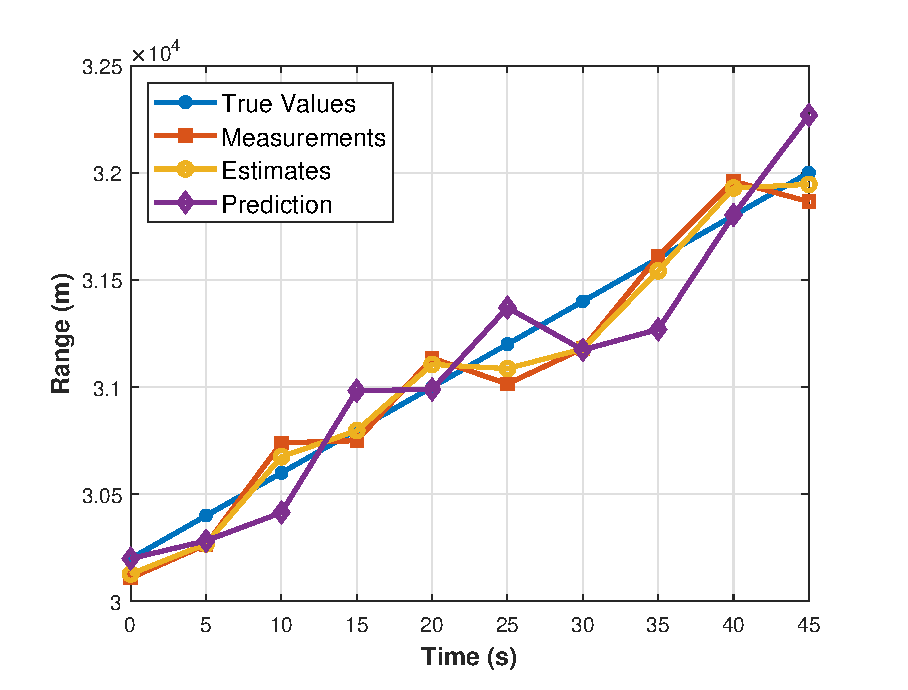
\includegraphics[width=0.9\textwidth]{Figures/Chapter1/ex2_estimationAlgorithm_alpha0.8_beta0.5.eps}
	    \label{fig:ex2_estimationAlgorithm_alpha0.8_beta0.5}
	    \vspace{-15pt}
	    \caption{$\alpha=0.8, \beta=0.5$}
	    \vspace{-8pt}
	\end{figure}
	"Smoothing" degree is much lower. The "current estimate" is very close to the measured values, and predicted estimate errors are high.
\end{columns}
\vspace{7pt}
\textcolor{blue}{$\alpha$ and $\beta$ values should depend on the measurement precision. If we use high precision equipment, we would prefer a high $\alpha$ and $\beta$ that follow measurements. In this case, the filter would quickly respond to a velocity change of the target. OTOH, if measurement precision is low, we prefer low  $\alpha$ and $\beta$. In this case, the filter smoothes the uncertainty (errors) in the measurements. However, the filter reaction to target velocity changes would be much slower.}

\texttt{\tiny [Code: a-b-c Filter/Ex2\_alpha-beta\_EstimationAlgorithm.m]}
\end{frame}
%-----------------------------------------------------
\subsubsection{Example~3: Tracking Accelerating Aircraft in 1D (Another Dynamic System)}
\begin{frame}{Example~3: Tracking Accelerating Aircraft in 1D}
\begin{columns}
    \column{0.5\textwidth}        
    This example tracks an aircraft moving with constant acceleration with the $\alpha-\beta$ filter.
    
    \vspace{5pt}
    
    In Example~2, aircraft was moving at a constant velocity of 40m/s. 
        \begin{figure}
	    \centering
	    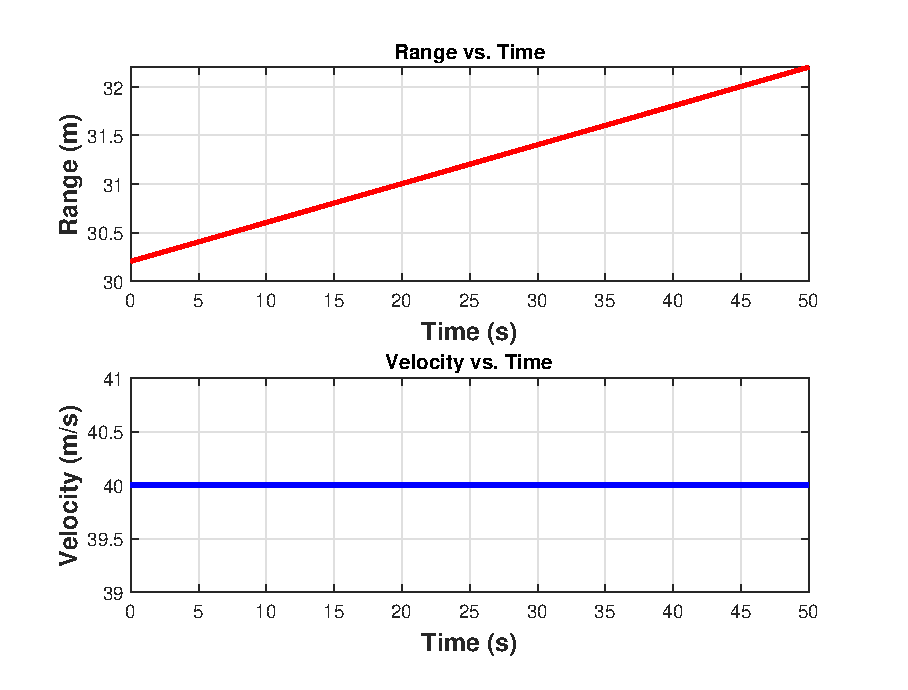
\includegraphics[width=1\textwidth]{Figures/Chapter1/ex3_preliminary1.eps}
	    \label{fig:ex3_preliminary1}
	    \vspace{-8pt}
	\end{figure}
        \texttt{\tiny [Code: a-b-c Filter/Ex3\_preliminary.m]}
    \column{0.5\textwidth} 
    
    Assume, a fighter aircraft moving at a constant velocity of 50\,m/s for 15 seconds. Then the aircraft accelerates with a constant acceleration of $8\,m/s^2$ for another 35 seconds.
        \begin{figure}
	    \centering
	    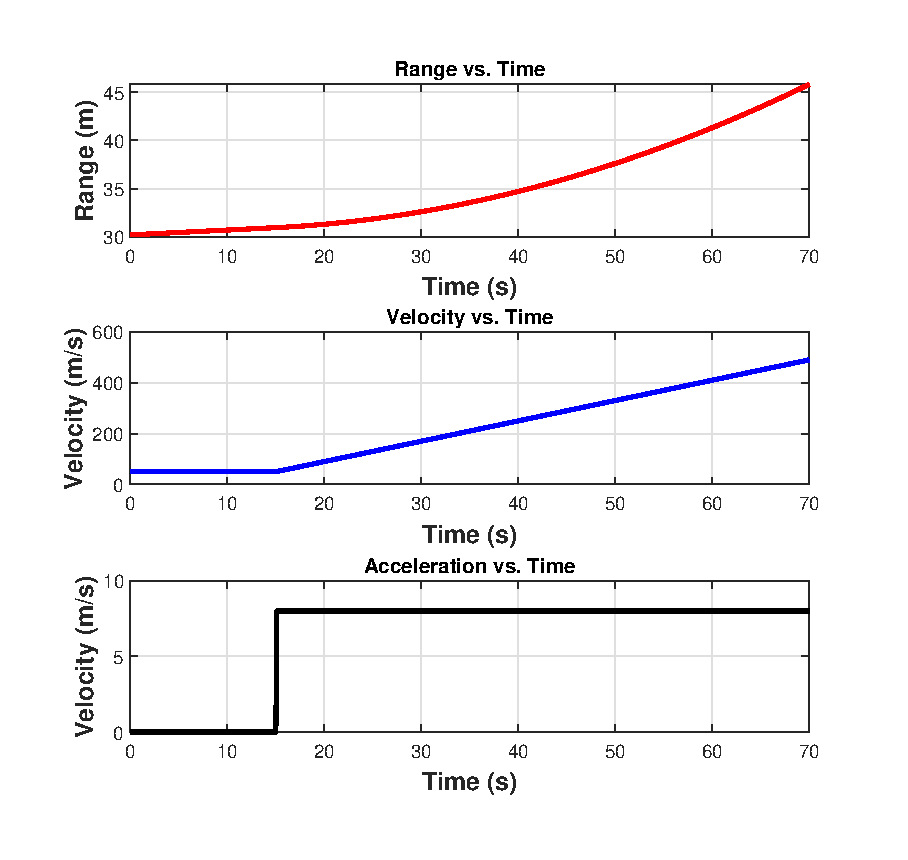
\includegraphics[width=1\textwidth]{Figures/Chapter1/ex3_preliminary2.eps}
	    \label{fig:ex3_preliminary2}
	    \vspace{-20pt}
	\end{figure}
	
Let's track this aircraft with the filter used in Example~2.
\end{columns}    
\end{frame}
%-----------------------------------------------------
\begin{frame}{Example~3: Tracking Accelerating Aircraft in 1D}
\textbf{Parameters:} $\alpha=0.2$, $\beta=0.1$, $\Delta t=5s$\\
\begin{columns}
    \column{0.5\textwidth}
    \begin{figure}
	    \centering
	    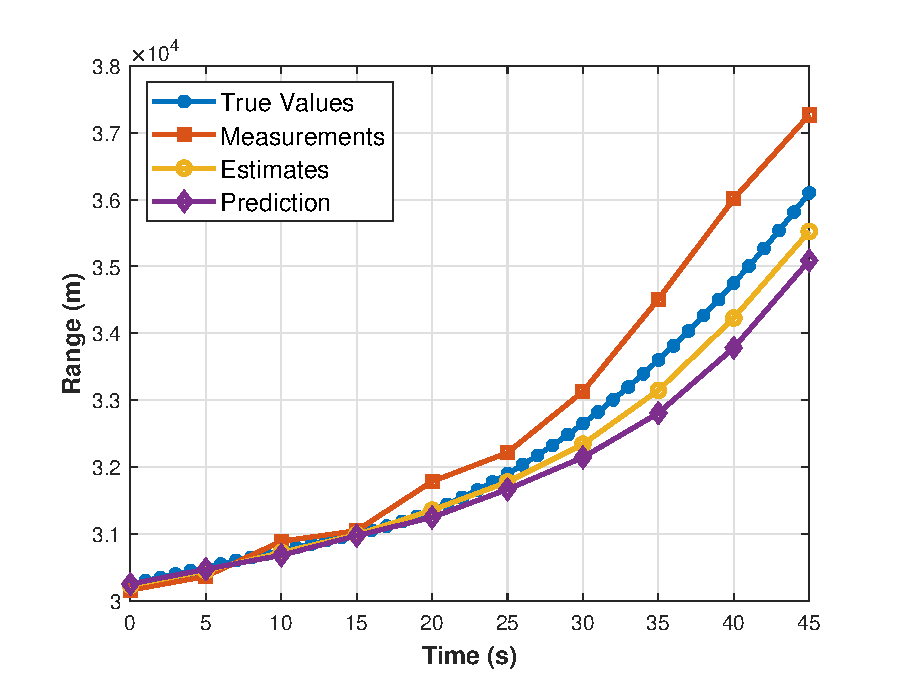
\includegraphics[width=0.9\textwidth]{Figures/Chapter1/ex3_estimationAlgorithm_range.eps}
	    \label{fig:ex3_estimationAlgorithm_range}
	   % \vspace{-20pt}
	\end{figure}
    
    \column{0.5\textwidth}
    \begin{figure}
	    \centering
	    \includegraphics[width=0.9\textwidth]{Figures/Chapter1/ex3_estimationAlgorithm_velocity.eps}
	    \label{fig:ex3_estimationAlgorithm_velocity}
	   % \vspace{-20pt}
	\end{figure}
\end{columns}
There is a constant gap between true or measured values and estimates. The gap is called a \textcolor{blue}{lag error}, or \textcolor{blue}{Dynamic error or Systematic error or Bias error or Truncation error}.
\vspace{5pt}

The lag error appears during the acceleration period. After the acceleration period, the filter closes the gap and converges toward the true value. However, a significant lag error can result in the target loss, which is unacceptable in certain applications, such as missile guidance or air defense.

\texttt{\tiny [Code: a-b-c Filter/Ex3\_alpha-beta\_EstimationAlgorithm.m]}
\end{frame}
%-----------------------------------------------------
\subsubsection{Example 4: Tracking the Accelerating Aircraft with the $\alpha-\beta-\gamma$ Filter}
\begin{frame}{Example 4: Tracking the Accelerating Aircraft with the $\alpha-\beta-\gamma$ Filter}
\begin{columns}
    \column{0.5\textwidth}
    \vspace{-20pt}
    \begin{center}
    \begin{minipage}{1\linewidth} % Adjust the minipage width as needed
    \begin{exampleblock}{\textbf{State Extrapolation Equations:}}
        \begin{align*}
            \hat{x}_{n+1,n} & = \hat{x}_{n,n} + \hat{\dot{x}}_{n,n}\Delta_t + \hat{\ddot{x}}_{n,n}\frac{\Delta_t^2}{2}\\
            \hat{\dot{x}}_{n+1,n} & = \hat{\dot{x}}_{n,n} + \hat{\ddot{x}}_{n,n}\Delta_t\\
            \hat{\ddot{x}}_{n+1,n} & = \hat{\ddot{x}}_{n,n}
        \end{align*}
    \end{exampleblock}
    \end{minipage}
\end{center}
    
    \column{0.5\textwidth}
    \vspace{-20pt}
    \begin{center}
    \begin{minipage}{1\linewidth} % Adjust the minipage width as needed
    \begin{exampleblock}{\textbf{State Update Equations:}}
    \begin{align*}
        \hat{x}_{n,n} & = \hat{x}_{n,n-1} + \alpha (z_n - \hat{x}_{n,n-1})\\
        \hat{\dot{x}}_{n,n} & = \hat{\dot{x}}_{n,n-1} + \beta\left(\frac{z_n - \hat{x}_{n,n-1}}{\Delta_t}\right)\\
        \hat{\ddot{x}}_{n,n} & = \hat{\ddot{x}}_{n,n-1} + \gamma\left(\frac{z_n - \hat{x}_{n,n-1}}{0.5\Delta_t^2}\right)
    \end{align*}
        \end{exampleblock}
    \end{minipage}
\end{center}
\end{columns}
\noindent\rule{5cm}{0.4pt}

    \textbf{Scenario from Example 3:} an aircraft that moves with a constant velocity of 50m/s for 15 seconds and then accelerates with a constant acceleration of $8m/s^2$ for another 35 seconds.
    
\noindent\rule{5cm}{0.4pt}

\begin{columns}    
    \column{0.5\textwidth}
    
    \vspace{4pt}
    \textbf{The $\alpha-\beta-\gamma$ filter parameters:}
    \begin{itemize}
        \item $\alpha=0.5$
        \item $\beta=0.4$
        \item $\gamma=0.1$
        \item $\Delta_t = 5s$
    \end{itemize}
    \column{0.5\textwidth}
    \textbf{Initialization:}
    \begin{itemize}
        \item $\hat{x}_{0,0} = 30,000$\,m
        \item $\hat{\dot{x}}_{0,0} = 50$\,m/s
        \item $\hat{\ddot{x}}_{0,0} = 0$\,m/$\text{s}^2$
    \end{itemize}    
\end{columns}    
\end{frame}

%-----------------------------------------------------
\begin{frame}{Example 4: Results}
\begin{columns}
    \column{0.6\textwidth}
    \begin{figure}
	    \centering
	    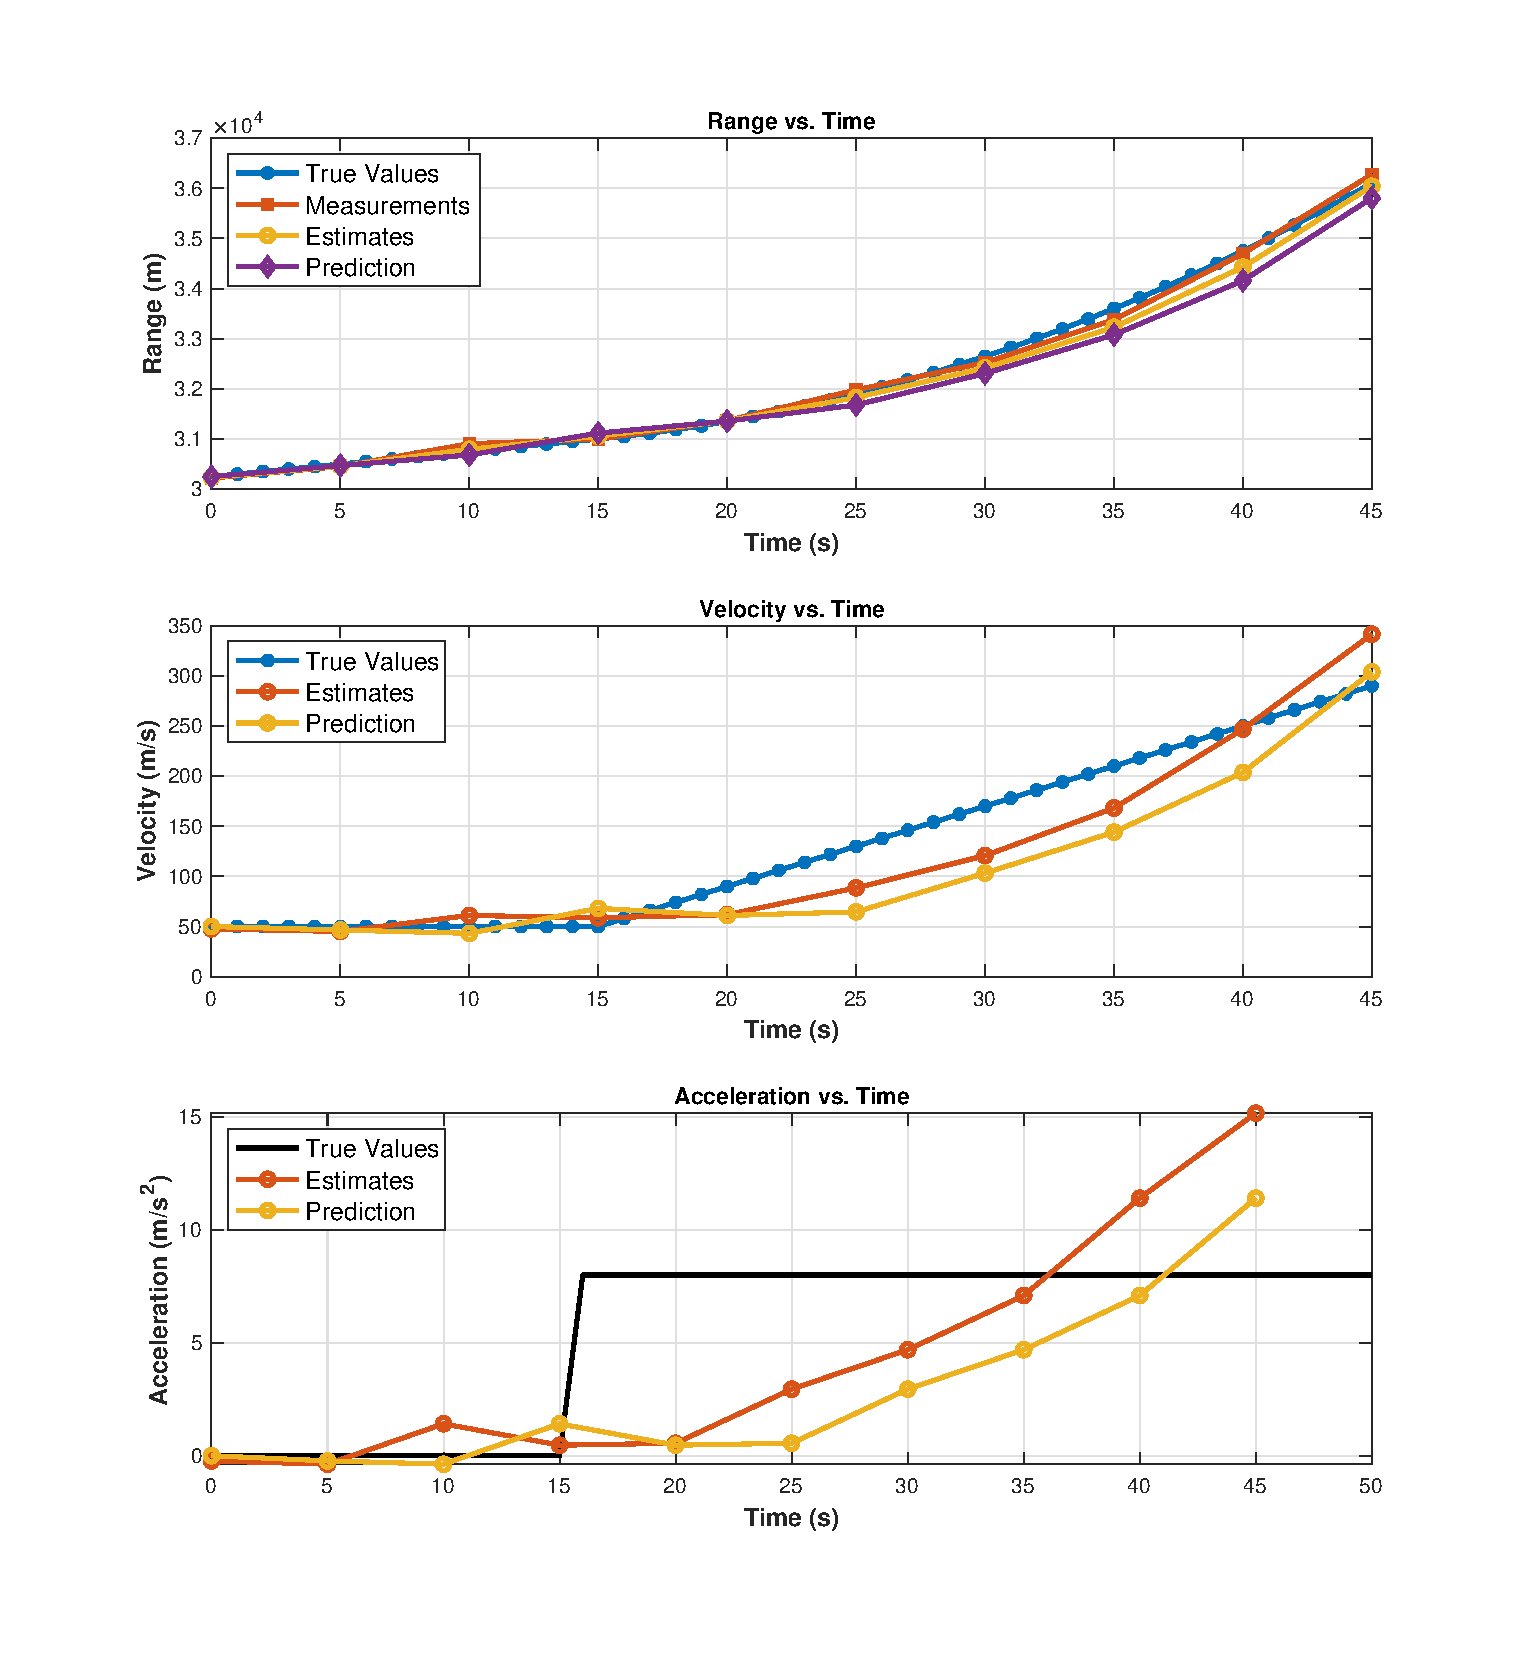
\includegraphics[width=0.9\textwidth]{Figures/Chapter1/ex4_estimationAlgorithm.eps}
	    \label{fig:ex4_estimationAlgorithm}
	   % \vspace{-20pt}
	\end{figure}
	\texttt{\tiny [Code: a-b-c Filter/Ex4\_alpha-beta-gamma\_EstimationAlgorithm.m]}
    \column{0.4\textwidth}
    \begin{itemize}
        \item The $\alpha-\beta-\gamma$ filter with dynamic model equations that include acceleration can track the target with constant acceleration and eliminate the lag error.
        \item But what happens in the case of a maneuvering target? The target can suddenly change the flight direction by making a maneuver. The target's dynamic model can also include a jerk (changing acceleration). 
        \item In such cases, the $\alpha-\beta-\gamma$  filter with constant $\alpha-\beta-\gamma$ coefficients produces estimation errors and, in some cases, loses the target track.
        \item \textcolor{blue}{The Kalman filter can handle uncertainty in the dynamic model.}
    \end{itemize}
\end{columns}    
\end{frame}
%-----------------------------------------------------
\begin{frame}{Summary of the $\alpha-\beta-\gamma$ Filter}

\begin{itemize}
    \item There are many types of $\alpha-\beta-\gamma$  filters, based on the same principle:
    \begin{itemize}
        \item The current state estimation is based on the state update equations.
        \item The following state estimation (prediction) is based on the dynamic model equations.
    \end{itemize}
    \item The main difference between these filters is the selection of weighting coefficients. \textcolor{blue}{Some filter types use constant, others compute at every iteration}
    \item Selection of parameters is discussed in detail in
        \begin{itemize}
            \item Dirk Tenne, Tarunraj Singh. "Optimal Design of $\alpha-\beta-\gamma$ Filters". State University of New York at Buffalo.
        \end{itemize}
    \item Another important issue is the initiation of the filter, i.e., providing the initial value for the first filter iteration.
\end{itemize}
    
\end{frame}

%-----------------------------------------------------
\begin{frame}{Most Popular $\alpha-\beta-\gamma$ Filters}
\begin{itemize}
    \item Wiener Filter
    \item Bayes Filter
    \item Fading-memory polynomial Filter
    \item Expanding-memory (or growing-memory) polynomial Filter
    \item Least-squares Filter
    \item Benedict–Bordner Filter
    \item Lumped Filter
    \item Discounted least-squares $\alpha-\beta$ Filter
    \item Critically damped $\alpha-\beta$ Filter
    \item Growing-memory Filter
    \item Kalman Filter
    \item Extended Kalman Filter
    \item Unscented Kalman Filter
    \item Extended Complex Kalman Filter
    \item Gauss-Hermite Kalman Filter
    \item Cubature Kalman Filter
    \item Particle Filter
\end{itemize}

    
\end{frame}

%-----------------------------------------------------
\subsection{One-Dimensional Kalman Filter without Process Noise}
\begin{frame}{One Dimensional Kalman Filter without Process Noise}
\begin{columns}

    \column{0.53\textwidth}
\textbf{Example~1: Gold Bar Weight Measurements.}\\
\textbf{Measurement errors:}
\begin{itemize}
    \item The different between true values and measurements; often described by variance ($\sigma^2$) for their randomness.
    \item The variance of the measurement errors could be provided by the scale vendor or \textcolor{blue}{derived by a calibration procedure}.
    \item The variance of the measurement errors is the \textcolor{blue}{measurement uncertainty}, denoted by $r$.
\end{itemize}
\textbf{Estimate error}
\begin{itemize}
    \item The difference between the estimates and the true values is the estimate error. 
    \item the estimate error becomes smaller and smaller as we make additional measurements, and it converges towards zero, while the estimated value converges towards the true value. 
    \item We don't know the estimate error, but we can estimate the uncertainty in estimate, denoted by $p$ (\textcolor{blue}{estimate variance}).
\end{itemize}
	\column{0.47\textwidth}
	            \begin{figure}
		    \centering
		   \includegraphics[width=1\textwidth]{Figures/Chapter1/ex1_estimationAlgorithm.eps}
		    \label{fig:ex1_estimationAlgorithm}
	    \end{figure}
	    \vspace{-12pt}
        \begin{figure}
		    \centering
		   \includegraphics[width=1\textwidth]{Figures/Chapter1/PDFs.png}
		    \label{fig:PDFs}
	    \end{figure}
\end{columns}
    
\end{frame}

%-----------------------------------------------------
\begin{frame}{State Prediction: Estimate Uncertainty Extrapolation or Covariance Extrapolation Equation (Eq.~3)}
Like state extrapolation, the estimate uncertainty extrapolation is done with the dynamic model equations.
\begin{columns}
    \column{0.5\textwidth}
        \begin{itemize}
            \item In Example~1 (gold bar weight measurement), the system's dynamics is constant. Thus, the estimate uncertainty extrapolation is:
            $$p_{n+1,n} = p_{n,n}$$
            where $p$ is the gold bar's weight estimate uncertainty
            
            \item In Example~2, the predicted target position is:
            \begin{align*}
	            \hat{x}_{n+1,n} & = \hat{x}_{n,n} + \Delta t \hat{\dot{x}}_{n,n}, & [\text{Aircraft range}]\\
	        \hat{\dot{x}}_{n+1,n} & = \hat{\dot{x}}_{n,n}, & [\text{Constant velocity}]
	    \end{align*}
	    i.e., the predicted position equals the current estimated position + the current estimated velocity x time. The predicted velocity equals the current velocity estimate (assuming a constant velocity model).
    
\end{itemize}
    \column{0.5\textwidth}
    \begin{itemize}
        \item The estimate uncertainty extrapolation would be:
        \begin{empheq}[box=\mymath]{gather*}
	            p_{n+1,n}^x = p_{n,n}^x + \Delta t^2 p_{n,n}^v,\\
	        p_{n+1,n}^v = p_{n,n}^v
	    \end{empheq}
	    where\\
	    $p^x$ is the position estimate uncertainty
	    $p^v$ is the velocity estimate uncertainty
    
        i.e., the predicted position estimate uncertainty equals the current position estimate uncertainty + current velocity estimate uncertainty $\times$ by time squared. The predicted velocity estimate uncertainty equals the current velocity estimate uncertainty (assuming a constant velocity model).
    \end{itemize}
    
\end{columns}


\end{frame}
%-----------------------------------------------------
\begin{frame}{State Prediction Illustration}
            \begin{figure}
		    \centering
		   \includegraphics[width=0.7\textwidth]{Figures/Chapter1/StatePredictionIllustration.png}
		    \label{fig:SatePrediction}
	    \end{figure}

    Note that for any normally distributed random variable $x$ with variance $\sigma^2$, $kx$ is distributed normally with variance $k^2\sigma^2$, therefore the time term in the uncertainty extrapolation equation is squared. 
\end{frame}
%-----------------------------------------------------
\begin{frame}{State Update: Kalman Gain Equation (Eq.4)}

To estimate the current state of the system, we combine two RVs:
    \begin{itemize}
        \item The prior state estimate (the current state estimate predicted at the previous state).
        \item The measurement
    \end{itemize}
    \begin{figure}
	 \centering
	 \includegraphics[width=0.5\textwidth]{Figures/Chapter1/StateUpdateIllustration.png}
	 \label{fig:SateUpdate}
    \end{figure}
\end{frame}

%-----------------------------------------------------
\begin{frame}{Kalman Gain cont...}
\textbf{The Kalman Filter is the optimal filter; it combines the prior state estimate with the measurements such that it minimizes the current state estimate uncertainty.} Derivation for 1D Kalman Filter:
\begin{columns}
    \column{0.5\textwidth}
        \begin{itemize}
            \item Given the measurement $z_n$ and the prior estimate $\hat{x}_{n,n-1}$, we want to find an optimum combined estimate $\hat{x}_{n,n}$ based on the measurement and the prior estimate.
            \item Which is actually a weighted mean of the prior estimate and the measurement:
            $$\hat{x}_{n,n}=k_1 z_n + k_2 \hat{x}_{n,n-1}$$
            Where $k_1$ and $k_2$ are the weights of the measurement and the prior estimate, i.e.,
            $$k_1 + k_2 = 1$$
            $$\hat{x}_{n,n}=k_1 z_n + (1-k_1) \hat{x}_{n,n-1}$$
            \item Since, for any normally distributed random variable $x$ with variance $\sigma^2$, $kx$ is distributed normally with variance $k\sigma^2$, thus:
            $${p}_{n,n}=k_1^2 r_n + (1-k_1)^2 {p}_{n,n-1}$$
    \end{itemize}
    \column{0.5\textwidth}
    where:\\
    $p_{n,n}$ is the variance of the optimum combined estimate $\hat{x}_{n,n}$\\
    $p_{n,n-1}$ is the variance of the prior estimate $\hat{x}_{n,n-1}$\\
    $r_n$ is the variance of the measurement $z_n$
    \begin{itemize}
        \item Since we are looking for an \textbf{optimum} estimate, we are interested to minimize $p_{n,n}$.
        \item To find $k_1$ that minimizes $p_{n,n}$, we differentiate $p_{n,n}$ with respect to $k_1$ and set the result to zero, i.e.,
        $$\frac{d p_{n,n}}{d k_1} = 2k_1r_n - 2 (1-k_1)p_{n,n-1}$$
        
        \boxed{
        $$\implies k_1 = \frac{p_{n,n-1}}{p_{n,n-1} + r_n}$$
        }
        \item Since the Kalman Gain yields the minimum variance estimate, the Kalman Filter is also called an \textbf{optimal filter}.
    \end{itemize}
\end{columns}
%-----------------------------------------------------

\end{frame}
\begin{frame}{State Update: Kalman Gain Equation (Eq.4)}

The Kalman Gain (denoted by $Kn$) is the weight given to the current state estimate and the measurements:

\begin{equation*}
    \boxed{K_n = \frac{\text{Uncertainty in Estimate}}{\text{Uncertainty in Estimate} + \text{Uncertainty in Measurement}} = \frac{p_{n,n-1}}{p_{n,n-1} + r_n}}
\end{equation*}
where $p_{n,n-1}$ is the extrapolated estimate uncertainty.
\begin{itemize}
    \item The Kalman Gain is a number between zero and one: $0\leq K_n \leq 1$
    \item Rewrite state update equation:
    $$\hat{x}_{n,n} = \hat{x}_{n,n-1} + K_n\left(z_n-\hat{x}_{n,n-1}\right) = \underbrace{(1-K_n)}_{\text{Current State Estimate Weight}}\hat{x}_{n,n-1} + \underbrace{K_n}_{\text{Measurement Weight}} z_n$$
    % \item The Kalman Gain ($K_n$) is the measurement weight, and the ($1-K_n$) term is the weight of the current state estimate.
    
    \item When the measurement uncertainty is large and the estimate uncertainty is low, the Kalman Gain is close to zero. Hence we give significant weight to the estimate and a small weight to the measurement.

\item OTOH, when the measurement uncertainty is low and the estimate uncertainty is large, the Kalman Gain is close to one. Hence we give a low weight to the estimate and a significant weight to the measurement.

\item If the measurement uncertainty equals the estimate uncertainty, then the Kalman gain equals 0.5.
\end{itemize}
\begin{exampleblock}{}
  {\large ``The Kalman gain tells how much the measurement changes the estimate.''}
\end{exampleblock}
\end{frame}

%-----------------------------------------------------
\begin{frame}{Estimate Uncertainty Update or Covariance Update Equation (Eq.~5)}
% \begin{columns}
    % \column{0.5\textwidth}        
    \textcolor{blue}{Estimate uncertainty update}, also called as \textcolor{blue}{Covariance Update Equation} is defined as
    \begin{empheq}[box=\mymath]{gather*}
        p_{n,n} = (1-K_n)p_{n,n-1},
    \end{empheq}
    where\\
    $K_n$~~~~~~is the Kalman Gain\\
    $p_{n,n-1}$ is the estimate uncertainty, calculated\\~~~~~~~~~during previous filter estimation\\
    $p_{n,n}$~~~~is estimate uncertainty of current state
    
    \vspace{5pt}
    \begin{itemize}
        \item Since $(1-K_n)\leq 1$, the estimate uncertainty is constantly getting smaller with each filter iteration. 
        
        \item When the measurement uncertainty is large, the Kalman gain is low. Therefore, the convergence of the estimate uncertainty would be slow. 
        
        \item However, the Kalman gain is high when the measurement uncertainty is small. Therefore, the estimate uncertainty would quickly converge towards zero.
    \end{itemize}
    
    % \column{0.5\textwidth}

% \end{columns}    
\end{frame}


\begin{frame}{Let's Put it All Together - Basic}
Like the $\alpha - \beta (-\gamma)$ filter, the Kalman filter utilizes the "Measure, Update, Predict" algorithm.
% \begin{columns}
    % \column{0.52\textwidth}
        \begin{figure}
		   \centering
		   \includegraphics[width=0.6\textwidth]{Figures/Chapter1/KalmanFilterAlgorithm.png}
		   \label{fig:PDFs}
	    \end{figure}
	    \vspace{-10pt}
	\textbf{Inputs:}
	\begin{itemize}
	    \item Initialization: (performed only once). Init. parameters can be provided by another system or process or an educated guess based on experience/theoretical knowledge. If not precise, Kalman filter tries to converge toward true value.
	       \begin{itemize}
	           \item Initial System State $(\hat{x}_{0,0})$
	           \item Initial Uncertainty $(p_{0,0})$
	       \end{itemize} 
	    \item Measurement:(performed at each filter cycle)
	        \begin{itemize}
	           \item Measured System State $(z_n)$
	           \item Measurement Uncertainty $(r_n)$. Usually,  $r_n$ is provided by the equipment vendor, or can be derived from equipment calibration. For example, the radar measurement uncertainty depends on several parameters such as SNR, beam width, bandwidth, time on target, clock stability, and more. While, every radar measurement has a different SNR, beam width, and time on target.
	       \end{itemize} 
	\end{itemize}
\end{frame}
%-----------------------------------------------------
\begin{frame}{Let's Put it All Together - Basic (Cont.)}
Contrary to the $\alpha - \beta (- \gamma)$ filter, the Kalman Filter treats measurements, current state estimation, and next state estimation (predictions) as normally distributed random variables.
% \begin{columns}
    % \column{0.52\textwidth}
        \begin{figure}
		   \centering
		   \includegraphics[width=0.6\textwidth]{Figures/Chapter1/KalmanFilterAlgorithm.png}
		   \label{fig:PDFs}
	    \end{figure}
	   % \vspace{-10pt}
	\textbf{Outputs:}
	\begin{itemize}
       \item System State Estimate $(\hat{x}_{n,n})$
       \item Estimate Uncertainty $(p_{n,n})$. 
       
       Since $p_{n,n} = (1-K_n)p_{n,n-1}$, $p_{n,n}$ is getting smaller with each filter iteration, as $(1-K_n)\leq1$. So it's up to us to decide how many measurements to take.
	\end{itemize}
\end{frame}


%-----------------------------------------------------
\begin{frame}{Let's Put it All Together - Basic (Cont.)}

% \begin{table}[]
%     \centering
%     \begin{tabular}{lll}
%         \toprule
%         \textbf{Equation} & \textbf{Equation Name} & \textbf{Alternative names} \\
%         \toprule
%         $\hat{x}_{n,n}= \hat{x}_{n,n-1} + K_n(z_n-\hat{x}_{n,n-1})$ & State Update & Filtering Equation \\ \hline
%         \begin{tabular}[c]{@{}l@{}} $\hat{x}_{n+1,n}= \hat{x}_{n,n} + \Delta t \hat{\dot{x}}_{n,n}$ \\ $\hat{\dot{x}}_{n+1,n} = \hat{\dot{x}}_{n,n}$ \\ (for constant velocity dynamics) \end{tabular} & State Extrapolation & \begin{tabular}[c]{@{}l@{}}Predictor Equation\\ Transition Equation\\ Prediction Equation \\ Dynamic Model \\ State Space Model \end{tabular} \\ \hline
%         $K_n = \dfrac{p_{n,n-1}}{p_{n,n-1} + r_n}$ & Kalman Gain & Weight Equation \\ \hline
%         $p_{n,n} = (1-K_n)p_{n,n-1}$ & Covariance Update & Corrector Equation \\ \hline
%         \begin{tabular}[c]{@{}l@{}} $p_{n+1,n} = p_{n,n}$ \\ (For constant dynamics) \end{tabular} & Covariance Extrapolation & Predictor Covariance Eq.\\
%         \bottomrule
%     \end{tabular}

    \begin{figure}
	   \centering
	   \includegraphics[width=0.75\textwidth]{Figures/Chapter1/KalmanFilterSummery.png}
	       \caption{Summary of Kalman Filter equations for a specific case (i.e., Example~2) }
    \label{tab:my_label}
	   \vspace{-10pt}
	   \end{figure}


%\end{table}
% }



\end{frame}
%-----------------------------------------------------

\begin{frame}{Let's Put it All Together - Detailed}

\begin{columns}
    \column{0.5\textwidth}
        \begin{figure}
	   \centering
	   \includegraphics[width=1\textwidth]{Figures/Chapter1/DetailedKalmanFilterAlgorithm.png}
	   \label{fig:DetailedKalmanFilterAlgorithm}
	   \vspace{-10pt}
	   \end{figure}

	\begin{itemize}
	    \item \textbf{Step 0: Initialization}
	       \begin{itemize}
	           \item Initial System State $(\hat{x}_{0,0})$
	           \item Initial Uncertainty $(p_{0,0})$
	       \end{itemize} 
	    \item \textbf{Step 1: Measurement}
	        \begin{itemize}
	           \item Measured System State $(z_n)$
	           \item Measurement Uncertainty $(r_n)$. 
	       \end{itemize} 
	\end{itemize}
		
	\column{0.5\textwidth} 
            \begin{itemize}
            \item \textbf{Step 2 - Inputs:} State Update (estimation of the system's current state). 
	        \begin{itemize}
	           \item Measured value $(z_n)$
	           \item Measurement Uncertainty $(r_n)$. 
	           \item Previous System State Estimate $(\hat{x}_{n,n-1})$
	           \item Estimate Uncertainty $(p_{n,n-1})$
	       \end{itemize} 
        \end{itemize}
	       Based on the inputs, the state update process calculates the Kalman Gain and provides two outputs:

	        \begin{itemize}
	            \item Current System State Estimate $(\hat{x}_{n,n})$
	            \item Current State Estimate Uncertainty $(p_{n,n})$
	        \end{itemize}
	    \begin{itemize} 
	        \item \textbf{Step 3: Prediction:}
	        \begin{itemize}
	            \item The prediction process extrapolates the current system state and uncertainty of the current system state estimate to the next system state, based on the system's dynamic model.
	            \item At the first filter iteration the initialization outputs are treated as the Previous State Estimate and Uncertainty.
	            \item The prediction outputs become the Previous State Estimate and Uncertainty on the following filter iterations.
	        \end{itemize}
	        
	            
	    \end{itemize}
\end{columns}	   	
\end{frame}

%-----------------------------------------------------

\begin{frame}{Kalman Gain Intuition - High Kalman Gain}
The Kalman Gain defines the weight of the measurement ($z_n$) and the weight of the previous estimate ($\hat{x}_{n,n-1}$) when forming a new estimate ($\hat{x}_{n,n}$).

\vspace{5pt}
A low measurement uncertainty relative to the estimate uncertainty would result in a high Kalman Gain (close to 1). Therefore the new estimate would be close to the measurement.
    \begin{figure}
	   \centering \includegraphics[width=0.65\textwidth]{Figures/Chapter1/HighKalmanGain.png}
	   \label{fig:HighKalmanGain}
	   \vspace{-10pt}
	\end{figure}
\end{frame}
%-----------------------------------------------------
\begin{frame}{Kalman Gain Intuition - Low Kalman Gain}
A high measurement uncertainty relative to the estimate uncertainty would result in a low Kalman Gain (close to 0). Therefore the new estimate would be close to the previous estimate.
    \begin{figure}
	   \centering
   \includegraphics[width=0.7\textwidth]{Figures/Chapter1/LowKalmanGain.png}
	   \label{fig:LowKalmanGain}
	   \vspace{-10pt}
	\end{figure}
\end{frame}

%-----------------------------------------------------
\subsubsection{Example~5: Estimating the Height of the Building}
\begin{frame}{Example~5: Estimating the Height of the Building}
\vspace{-5pt}
We would like to estimate the height of a building using a very imprecise altimeter. The building height doesn't change over time, at least during the short measurement process.

\begin{columns}
    \column{0.5\textwidth}        
    \begin{itemize}
        \item The true building height is 50 meters.
        \item The altimeter measurement error (standard deviation) is 5 meters.
        \item The ten measurements are: 48.54m, 47.11m, 55.01m, 55.15m, 49.89m, 40.85m, 46.72m, 50.05m, 51.27m, 49.95m.
    \end{itemize}
    \textbf{ITERATION ZERO}
    \begin{itemize}
        \item \textbf{Initialization:}
        \begin{itemize}
            \item Estimated build height
            $$\hat{x}_{0,0} = 60m$$
            \item Estimate uncertainty with std. $\sigma = 15m$,
            $$p_{0,0} = 225$$
        \end{itemize}
        \item \textbf{Prediction:}
            \begin{itemize}
                \item Since Dynamic Model is constant
                $$\hat{x}_{1,0}= \hat{x}_{0,0} = 60$$
                \item The extrapolated estimate uncertainty (variance) also doesn't change:
                $$\hat{p}_{1,0}= \hat{p}_{0,0} = 225$$
            \end{itemize}
    \end{itemize}
    \column{0.5\textwidth}        
    \textbf{FIRST ITERATION}
    \begin{itemize}
        \item \textbf{Step~1: Measure:}
            \begin{itemize}
                \item The first measurement is
                $$z_1 = 48.54m$$
                \item The measurement uncertainty (since $\sigma=5$)
                $$r_1 = 25$$
            \end{itemize}
        \item \textbf{Step~2: Update:}
            \begin{itemize}
                \item Kalman gain
                $$K_1 = \frac{p_{1,0}}{p_{1,0} + r_n} = 0.9$$
                \item Estimating the current state:
                $$\hat{x}_{1,1} = \hat{x}_{1,0} + K_1 (z_1 - \hat{x}_{1,0}) = 49.69m$$
                \item  Current estimate uncertainty
                $$p_{1,1} = (1-K_1) p_{1,0} = 22.5$$
            \end{itemize}
        \item \textbf{Step~3: Predict:}
            \begin{itemize}
                \item For constant dynamic model,  
                $$\hat{x}_{2,1} = \hat{x}_{1,1} = 49.69m$$
                $$p_{2,1} = p_{1,1} = 22.5$$
                
            \end{itemize}
    \end{itemize}
\end{columns}
    
    
\end{frame}


%-----------------------------------------------------
\begin{frame}{Example~5: Estimating the Height of the Building --- Results}
\begin{columns}
\vspace{-10pt}
    \column{0.5\textwidth}
    \begin{figure}
	   \centering
	   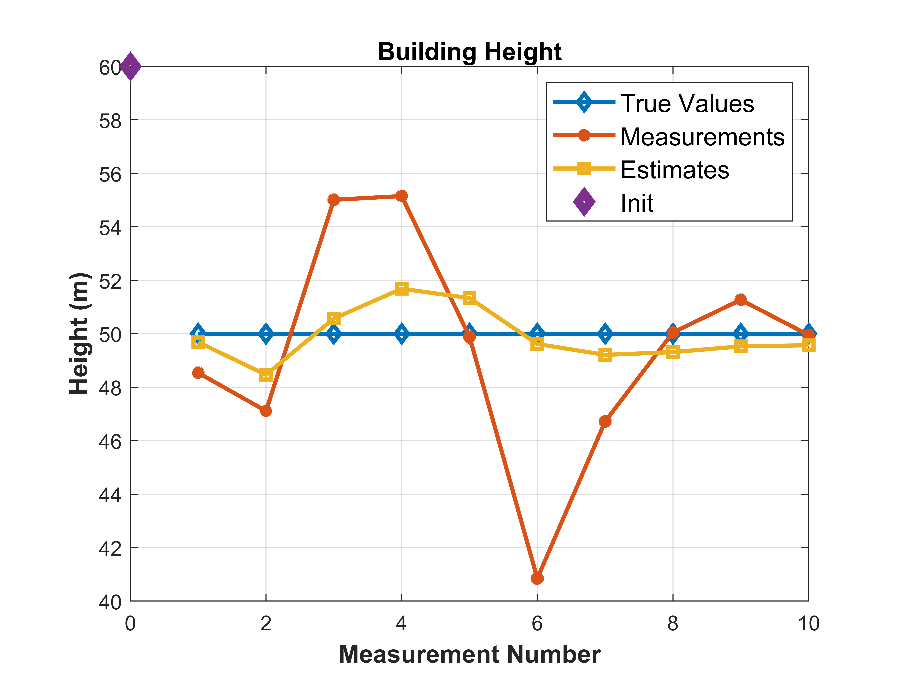
\includegraphics[width=0.6\textwidth]{Figures/Chapter1/ex5_FirstKalmanFilter_H_Estimate.eps}
	   \label{fig:ex5_FirstKalmanFilter_H_Estimate}
	   \vspace{-10pt}
	\end{figure}
	The estimated value converges to about 49.5 meters after 7 measurements.
	
	\begin{figure}
	   \centering
	   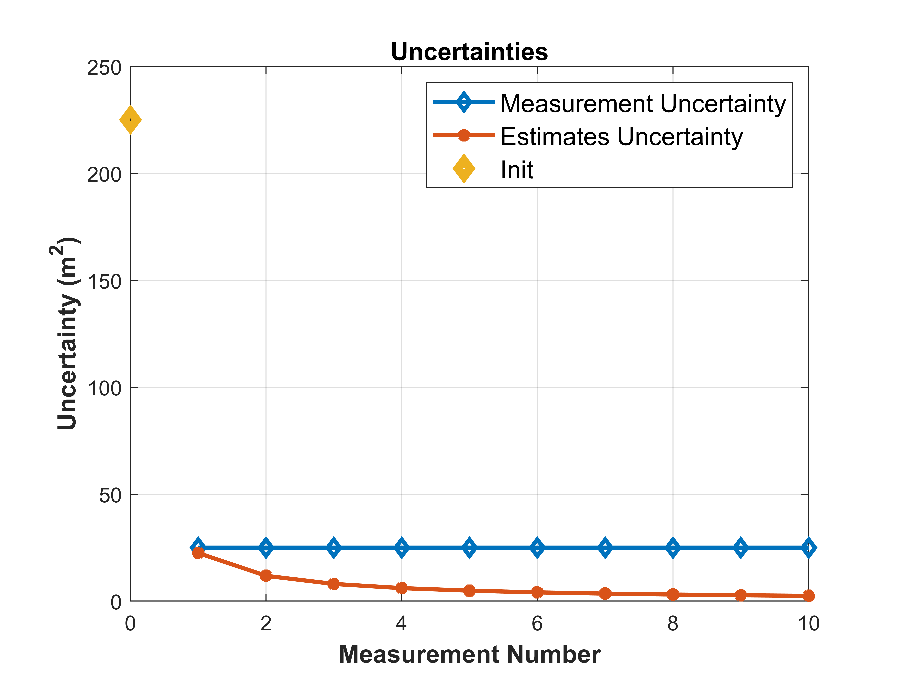
\includegraphics[width=0.6\textwidth]{Figures/Chapter1/ex5_FirstKalmanFilter_Estimate_Uncertainties.eps}
	   \label{fig:ex5_FirstKalmanFilter_Estimate_Uncertainties}
	   \vspace{-10pt}
	\end{figure}
	At 1st filter iteration, the estimate uncertainty is close to the measurement uncertainty and quickly decreases. After 10 measurements, the estimate uncertainty ($\sigma^2$) is 2.47, i.e., the estimate error std is: $\sigma =\sqrt(2.47)=1.57m$.
    \column{0.5\textwidth}
    
    \begin{figure}
	   \centering
	   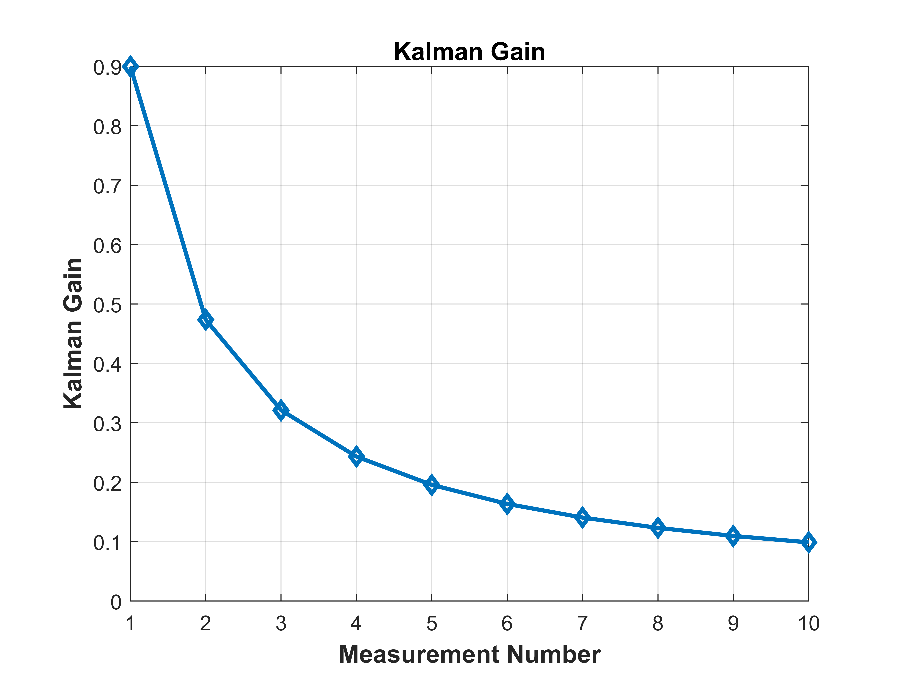
\includegraphics[width=0.8\textwidth]{Figures/Chapter1/ex5_FirstKalmanFilter_KalmanGain.eps}
	   \label{fig:ex5_FirstKalmanFilter__KalmanGain}
	   \vspace{-10pt}
	\end{figure}
	
\textbf{Summary:}	
\begin{itemize}
    \item The Kalman Gain is dynamic and depends on the precision of the measurement device.
    \item The initial value used by the Kalman Filter is not precise. Therefore, the measurement weight in the State Update Equation is high, and the estimate uncertainty is high.
    \item With each iteration, the measurement weight is lower; therefore, the estimate uncertainty is lower.
\end{itemize}
	
\end{columns}    
\end{frame}

%-----------------------------------------------------
\begin{frame}{Example~5: Estimating the Height of the Building --- Results}

One can define accuracy criteria based on the specific application requirements. The
typical accuracy criteria are: \textcolor{blue}{Maximum error, Mean error, Root Mean Square Error (RMSE)}.


Assume that for a building height measurement application, there is a requirement for 95\% confidence.
\begin{columns}
    \column{0.5\textwidth} 
        \begin{figure}
	   \centering
	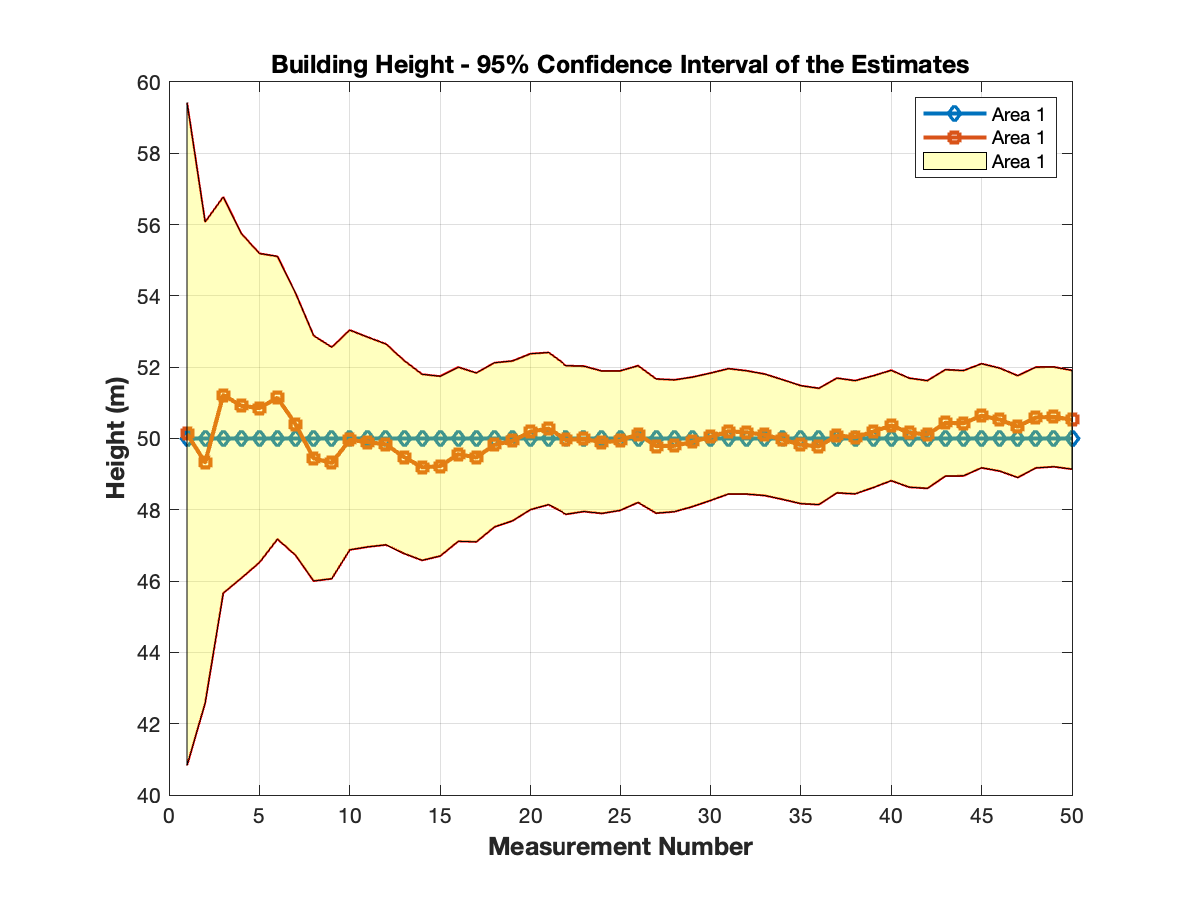
\includegraphics[width=1\textwidth]{Figures/Chapter1/ex5_FirstKalmanFilter_highUncertainty.eps}  \label{fig:ex5_FirstKalmanFilter_highUncertainty}
  \vspace{-20pt}
    \caption{High Uncertainty: $r=5$\,m}
    %\vspace{-5pt}
    \end{figure}
    \column{0.5\textwidth}
        \begin{figure}
	   \centering
	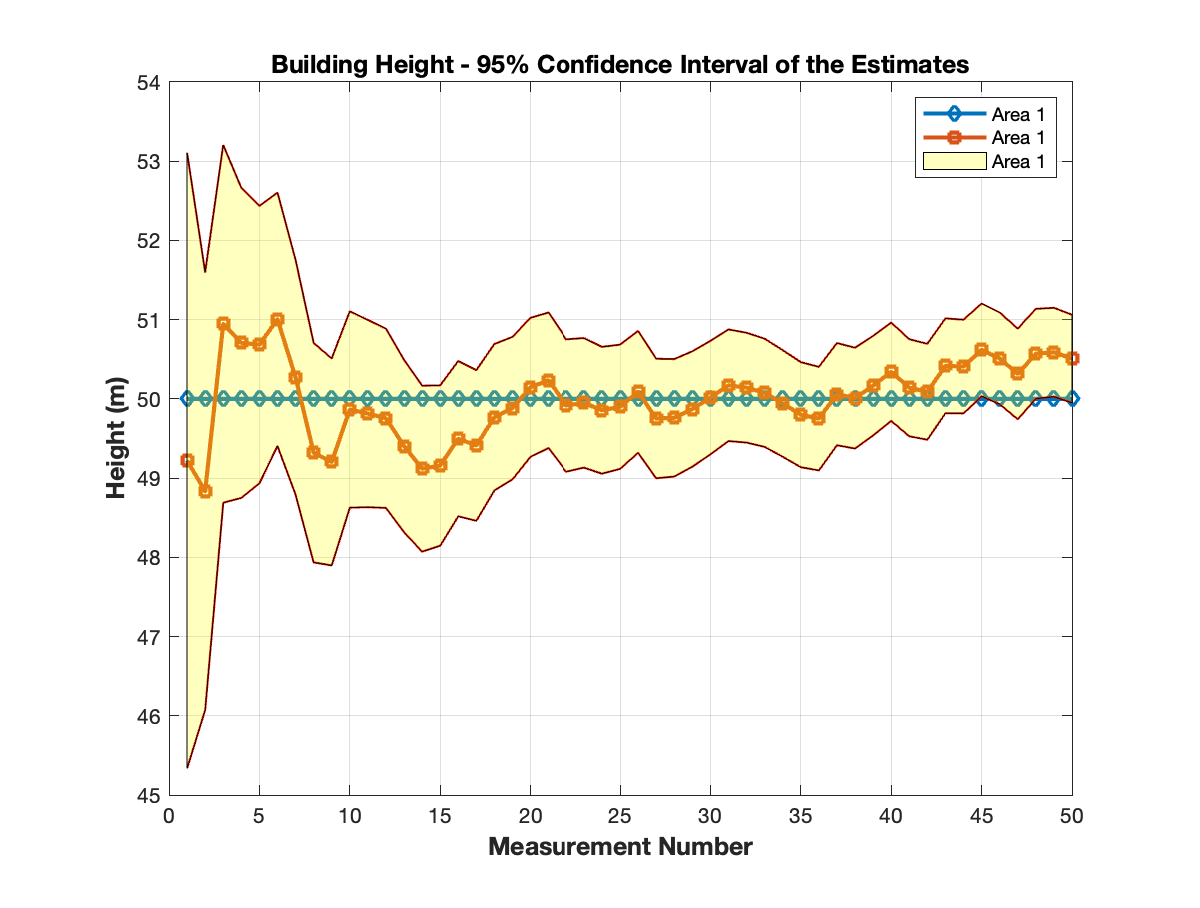
\includegraphics[width=1\textwidth]{Figures/Chapter1/ex5_FirstKalmanFilter_highUncertainty_r2.eps}  \label{fig:ex5_FirstKalmanFilter_highUncertainty}
  \vspace{-20pt}
 \caption{High Uncertainty: $r=2$\,m}
   % \vspace{-5pt}
    \end{figure}
\end{columns}

With measurement uncertainty $r=2$\,m, 2 out of 50 samples slightly exceed the 95\% confidence region; satisfying our requirements of desired estimate uncertainty.

\texttt{\tiny [Code: 1D KF/Ex5\_FirstKalmanFilter.m]}
\end{frame}
%-----------------------------------------------------

\subsection{One-Dimensional Kalman Filter with Process Noise}
\begin{frame}{Complete Model of 1D Kalman Filter including Process Noise}
To complete the one-dimensional Kalman Filter model, we need to add the process noise variable to the Covariance Extrapolation Equation.

\textbf{The Process Noise:}

\begin{itemize}
    \item In the real world, there are uncertainties in the system dynamic model. For example, 
    \begin{itemize}
        \item  When estimating the resistance value of the resistor, we assume a constant dynamic model, i.e., the resistance doesn't change between the measurements. However, the resistance can change slightly due to the fluctuation of the environment temperature.
        
        \item When tracking ballistic missiles with radar, the uncertainty of the dynamic model includes random changes in the target acceleration. 
        
        \item The uncertainties are much more significant for an aircraft due to possible aircraft maneuvers.
        
        \item On the other hand, when estimating the location of a static object using a GPS receiver, the uncertainty of the dynamic model is zero since the static object doesn't move.
    \end{itemize}
    \item The uncertainty of the dynamic model is called the \textcolor{blue}{Process Noise}. In the literature, it is also called \textit{plant noise, driving noise, dynamics noise, model noise, and system noise}. The process noise produces estimation errors.
    
    \item The \textcolor{blue}{Process Noise Variance} is denoted by the letter $q$.
    
    \item The Covariance Extrapolation Equation shall include the Process Noise Variance.
    
    \item For example, the Covariance Extrapolation Equation for constant dynamics is:
    $$p_{n+1,n} = p_{n,n} + q_n$$
    Note: The State Extrapolation Equation and the Covariance Extrapolation Equation depend on the system dynamics.
\end{itemize}
    
\end{frame}



\begin{frame}{Example~6: Estimating the Temperature of the Liquid in a Tank} 
\begin{columns}
    \column{0.5\textwidth}        
    We assume that at a steady state, the liquid temperature is constant. However, some fluctuations in the true liquid temperature are possible. 
    \begin{figure}
        \centering
        \includegraphics[width=0.5\textwidth]{Figures/Chapter1/ex6_liquid_temperature.png}
        \label{fig:ex6_liquid_temperature}
    \end{figure}
    
    
    We can describe the system dynamics by the following equation:
    
    $$x_n = T + w_n$$
    where\\
    $T$~~is the constant temperature\\
    $w_n$~is a random process noise with variance $q$
    
    \textbf{Assumptions:}
    \begin{itemize}
        \item Tanks true temperature of 50 degrees Celsius
    \end{itemize}
    
    \column{0.5\textwidth}  
    \begin{itemize}
        \item We assume that the model is accurate. Thus, we set the process noise variance, $q=0.0001$.
        \item The measurement error (standard deviation) is 0.1 degrees Celsius.
        \item The measurements are taken every 5 seconds.
        \item The true liquid temperature values at the measurement points are (in degrees Celsius): 49.979, 50.025, 50, 50.003, 49.994, 50.002, 49.999, 50.006, 49.998, and 49.991.
        \item The measurements are (in degrees Celsius): 49.95, 49.967, 50.1, 50.106, 49.992, 49.819, 49.933, 50.007, 50.023, and 49.99.
    \end{itemize}
\end{columns}

    
\end{frame}

%-----------------------------------------------------
\subsubsection{Example~6: Estimating the Temperature of the Liquid in a Tank} 
\begin{frame}{Example~6: Estimating the Temperature of the Liquid in a Tank} 
\begin{columns}
    \column{0.5\textwidth}        
       \textbf{ITERATION ZERO}
    \begin{itemize}
        \item \textbf{Initialization:}
        \begin{itemize}
            \item We don't know the true temperature of the liquid in a tank; our estimate (or guess) is
            $$\hat{x}_{0,0} = 10^o C$$
            \item Estimate uncertainty with std. $\sigma = 100$,
            $$p_{0,0} = \sigma^2 = 10,000$$
        \end{itemize}
        \item \textbf{Prediction:}
            \begin{itemize}
                \item Since our model has constant dynamics, the predicted estimate is equal to the current estimate:
                $$\hat{x}_{1,0}= \hat{x}_{0,0} = 10^oC$$
                \item The extrapolated estimate uncertainty (variance):
                $$\hat{p}_{1,0}= \hat{p}_{0,0} + q = 10000 + 0.0001$$
            \end{itemize}
    \end{itemize}
    \column{0.5\textwidth}
        \textbf{FIRST ITERATION}
    \begin{itemize}
        \item \textbf{Step~1: Measure:}
            \begin{itemize}
                \item The first measurement is
                $$z_1 = 49.95^oC$$
                
                \item The measurement uncertainty (since $\sigma=0.1$)
                $$r_1 = 0.01$$
            \end{itemize}
        \item \textbf{Step~2: Update:}
            \begin{itemize}
                \item Kalman gain
                $$K_1 = \frac{p_{1,0}}{p_{1,0} + r_n} = 0.999999~[\approx 1]$$
                \item Estimating the current state:
                $$\hat{x}_{1,1} = \hat{x}_{1,0} + K_1 (z_1 - \hat{x}_{1,0}) = 49.95^o C$$
                \item  Current estimate uncertainty
                $$p_{1,1} = (1-K_1) p_{1,0} = 0.01$$
            \end{itemize}
        \item \textbf{Step~3: Predict:}
            \begin{itemize}
                \item For constant dynamic model,  
                $$\hat{x}_{2,1} = \hat{x}_{1,1} = 49.95^o C$$
                $$p_{2,1} = p_{1,1} + q = 0.0101$$
                
            \end{itemize}
    \end{itemize}
\end{columns}
    
\end{frame}

%-----------------------------------------------------
\begin{frame}{Example~6: Estimating the Temperature of the Liquid in a Tank --- Results} 
\begin{columns}
    \column{0.5\textwidth}
    \begin{itemize}
        \item The estimated value converges toward the true value.
        \item The estimate uncertainty quickly goes down. After 10 measurements, the estimate uncertainty is $\sigma^2=0.0013$, i.e., the estimate error std is: $\sigma=0.036^oC$.
        \item So we can say that the liquid temperature estimate is: $49.988 \pm 0.036^oC$.
        \item \textbf{Summary:} Although the system dynamics include a random process noise, the Kalman Filter can provide a good estimation.
    \end{itemize}
    \vspace{-10pt}
    \begin{figure}
        \centering
        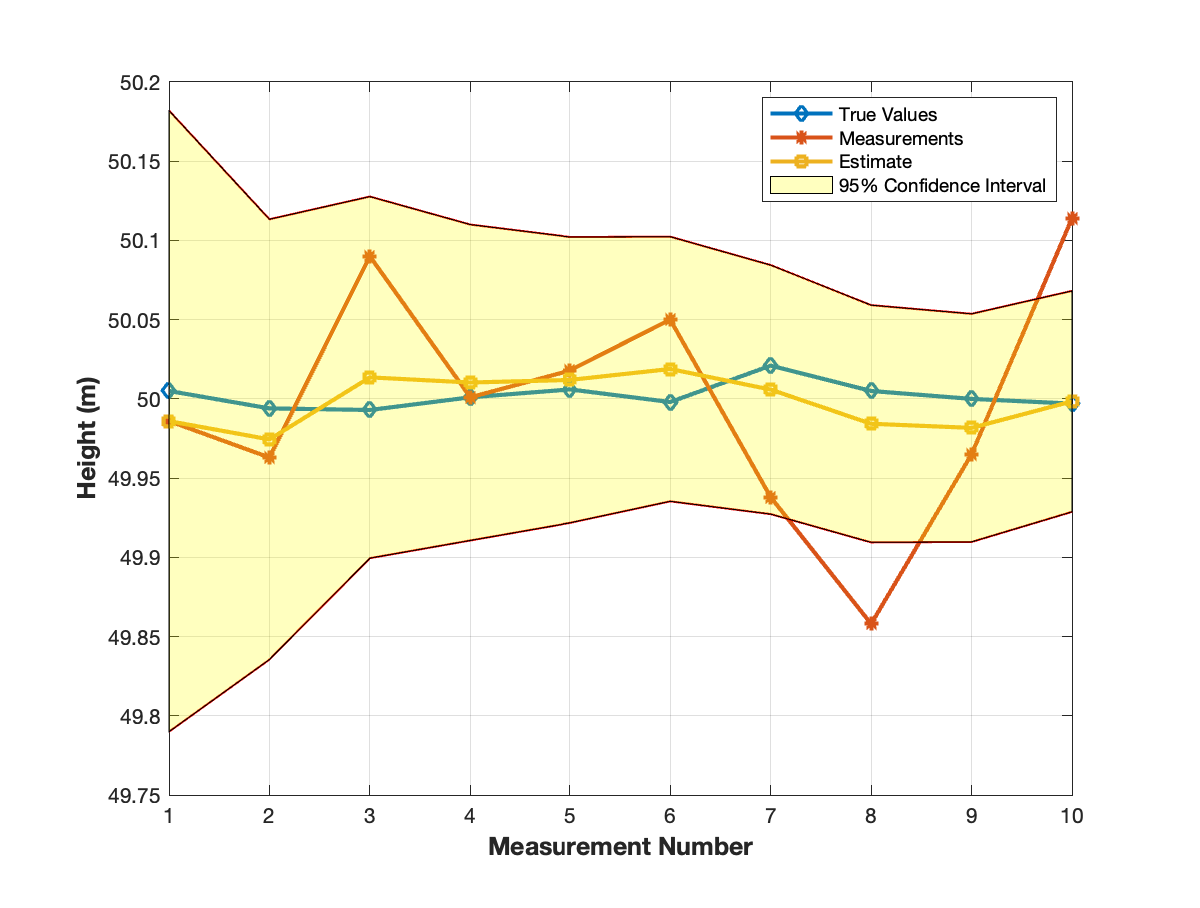
\includegraphics[width=0.8\textwidth]{Figures/Chapter1/ex6_KalmanFilter_ProcessNoise_95CI.eps}
\label{fig:ex6_KalmanFilter_ProcessNoise_95CI}
    \end{figure}
    \column{0.5\textwidth}
    \begin{figure}
        \centering
        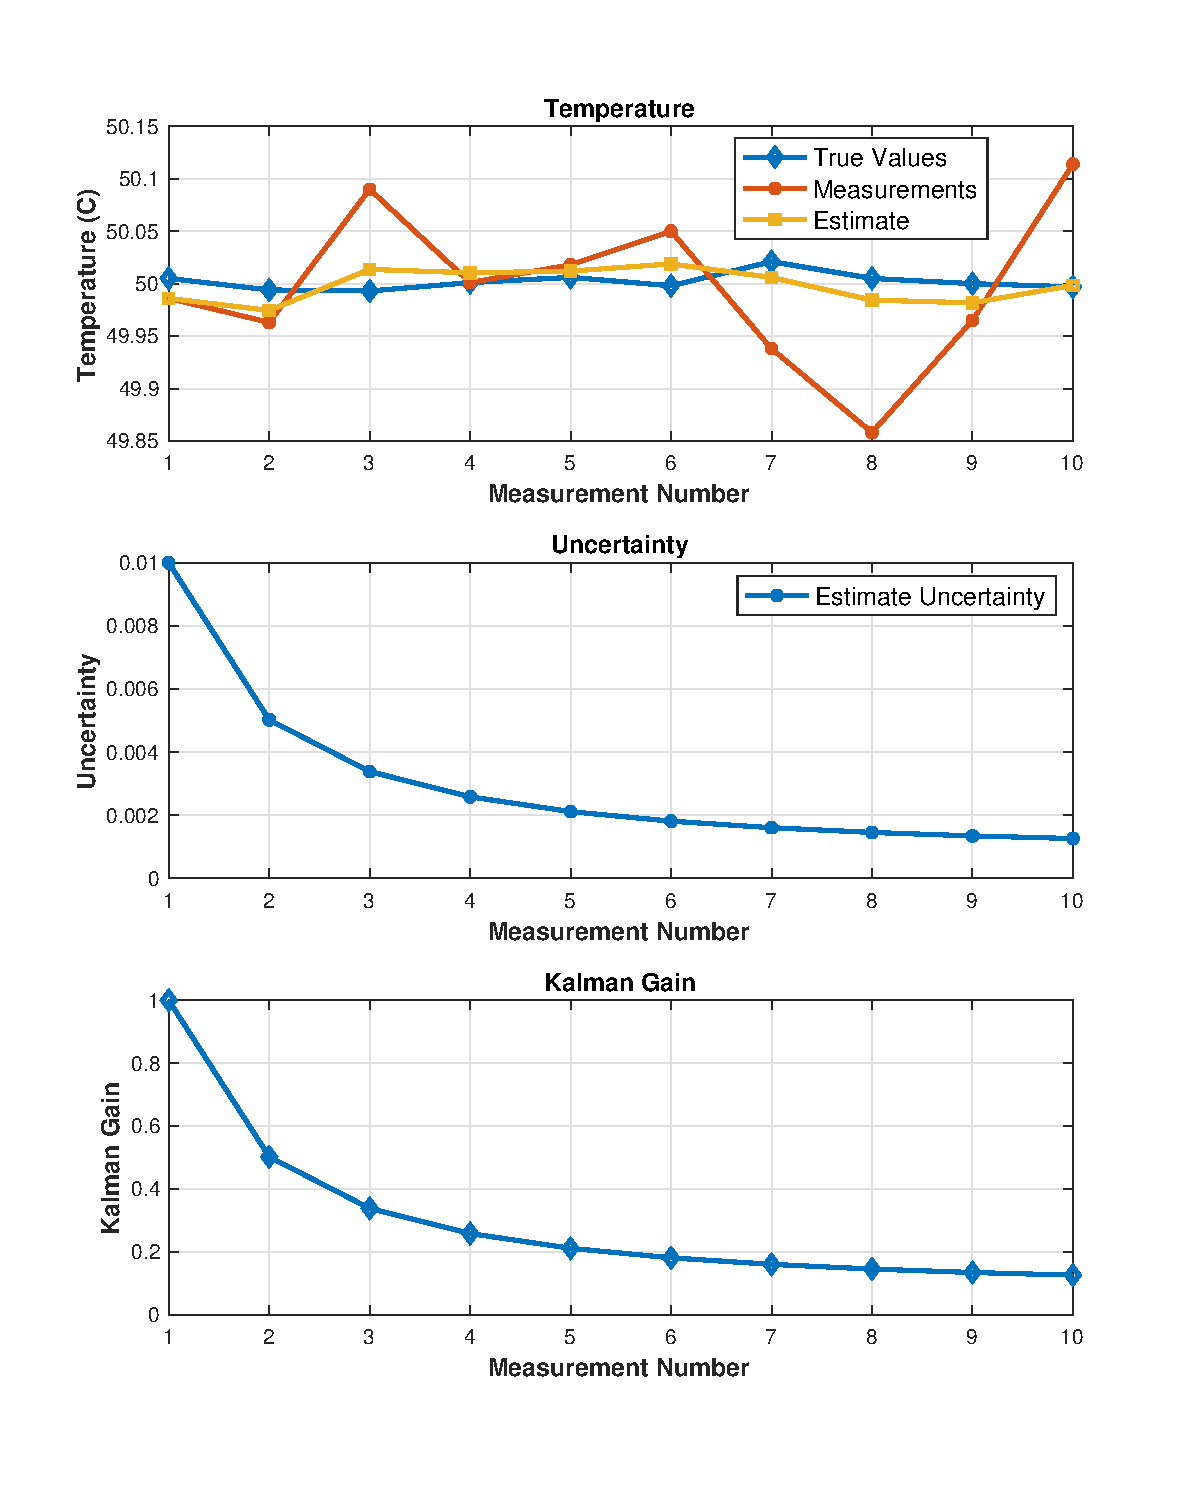
\includegraphics[width=1\textwidth]{Figures/Chapter1/ex6_KalmanFilter_ProcessNoise.eps}
        \label{fig:ex6_KalmanFilter_ProcessNoise}
        \vspace{-25pt}
    \end{figure}
    \texttt{\tiny [Code: 1D KF/Ex6\_KalmanFilter\_ProcessNoise.m]}
\end{columns}
\end{frame}
%----------------------------------------------------- 
\subsubsection{Example~7: Estimating the Temperature of a Heating Liquid in a Tank I} 
\begin{frame}{Example~7: Estimating the Temperature of a Heating Liquid in a Tank I} 
\begin{columns}
    \column{0.5\textwidth}        
    \begin{itemize}
        \item Let's estimate the temperature of a liquid in a tank as in Example~6. However, in this case, the dynamic model of the system is not constant--- the liquid is heating at a rate of $0.1^oC/sec$.
        \item Parameters are same as in Example~6.
        \item The dynamic model of the system is constant. Although the true dynamic model of the system is not constant (since the liquid is heating), we treat the system as a system with a constant dynamic model (the temperature doesn't change)
        \item The true liquid temperature values at the measurement points are: 50.479, 51.025, 51.5, 52.003, 52.494, 53.002, 53.499, 54.006, 54.498, and 54.991.
        \item The measurements are: 50.45, 50.967, 51.6, 52.106, 52.492, 52.819, 53.433, 54.007, 54.523, and 54.99.
        \item Kalman Filter has failed to provide a reliable estimation as there is a lag error in the estimation.
    \end{itemize}    
    \column{0.5\textwidth}
    \vspace{-5pt}
    \begin{figure}
        \centering
        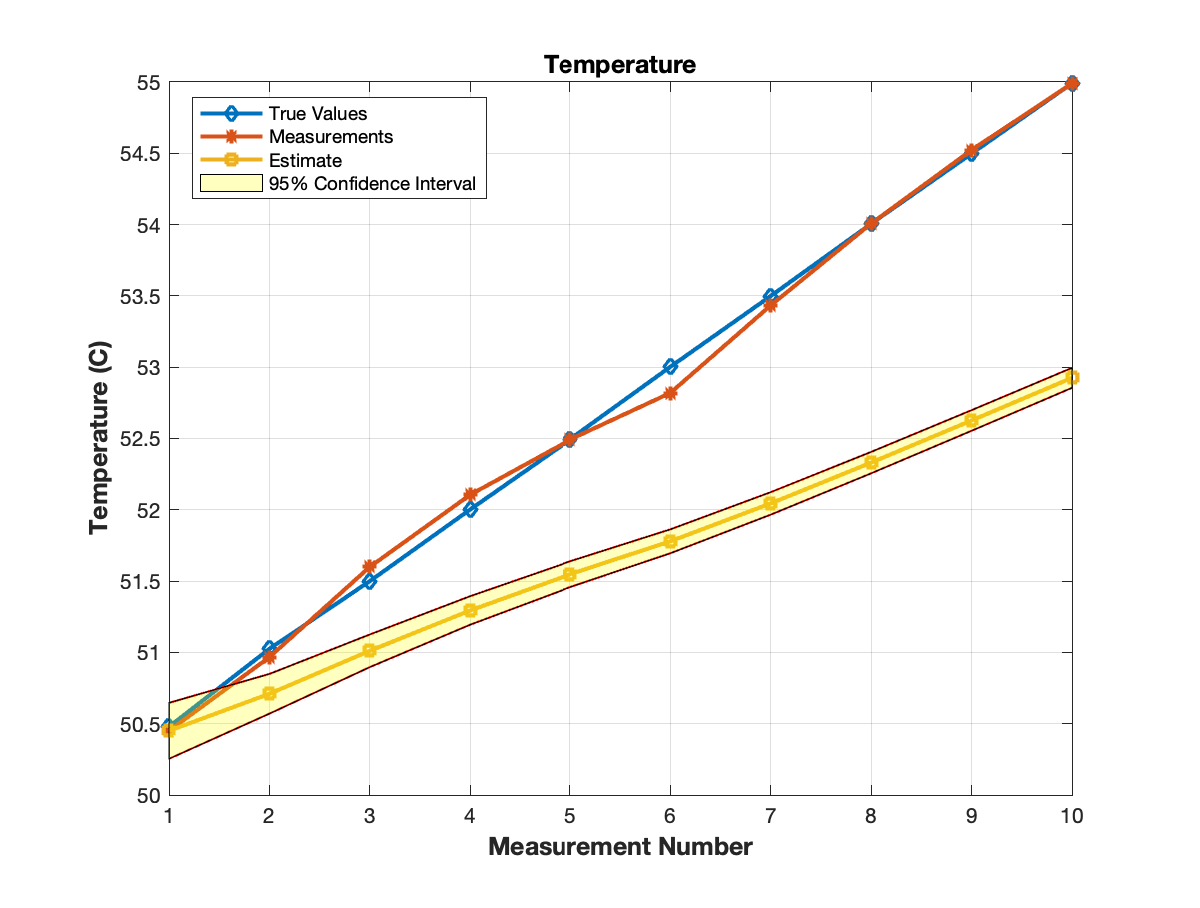
\includegraphics[width=0.7\textwidth]{Figures/Chapter1/ex7_KalmanFilter_ProcessNoise_I.eps}
        \label{fig:ex7_KalmanFilter_ProcessNoise_I}
        \vspace{-10pt}
    \end{figure}
    \begin{itemize}
     \item \textbf{Two Reason for the constant lag error:}  
    % The lag error is caused by the wrong dynamic model and process model definitions.
        \begin{itemize}
            \item The dynamic model doesn't fit the case.
            \item  Process noise is very low ($q=0.0001$) while the true temperature fluctuations are much more significant.
        \end{itemize}
        \item Two possible ways to fix the lag error:    
            \begin{itemize}
                \item If we know that the liquid temperature can change linearly, we can define a new model that considers that. \textit{What of the temperature change cannot be modeled?}
                \item If the model is not well defined, we can adjust the process model reliability by increasing the process noise ($q$).
            \end{itemize}
    \end{itemize}
            \texttt{\tiny [Code: 1D KF/Ex7\_KalmanFilter\_ProcessNoise\_I.m]}
\end{columns}
\end{frame}

%-----------------------------------------------------
\subsubsection{Example~8: Estimating the Temperature of a Heating Liquid in a Tank II}
\begin{frame}{Example~8: Estimating the Temperature of a Heating Liquid in a Tank II} 
\begin{columns}
    \column{0.5\textwidth}        
    This example is similar to the previous example, with only one change. Since our process is not well-defined, we increase the process uncertainty ($q$) from 0.0001 to 0.15.
    \begin{itemize}
        \item Due to the high process uncertainty, the measurement weight is much higher than the weight of the estimate. Thus, the Kalman Gain is high, and it converges to 0.94.
        \item We can eliminate the lag error by setting a high process uncertainty. However, since our model is not well-defined, we get noisy estimates that are almost equal to the measurements, and we miss the goal of the Kalman Filter.
        \item The best Kalman Filter implementation would involve a model that is very close to reality, leaving little room for process noise. However, a precise model is not always available 
    \end{itemize}
    
    \column{0.5\textwidth}   
    \begin{figure}
        \centering
        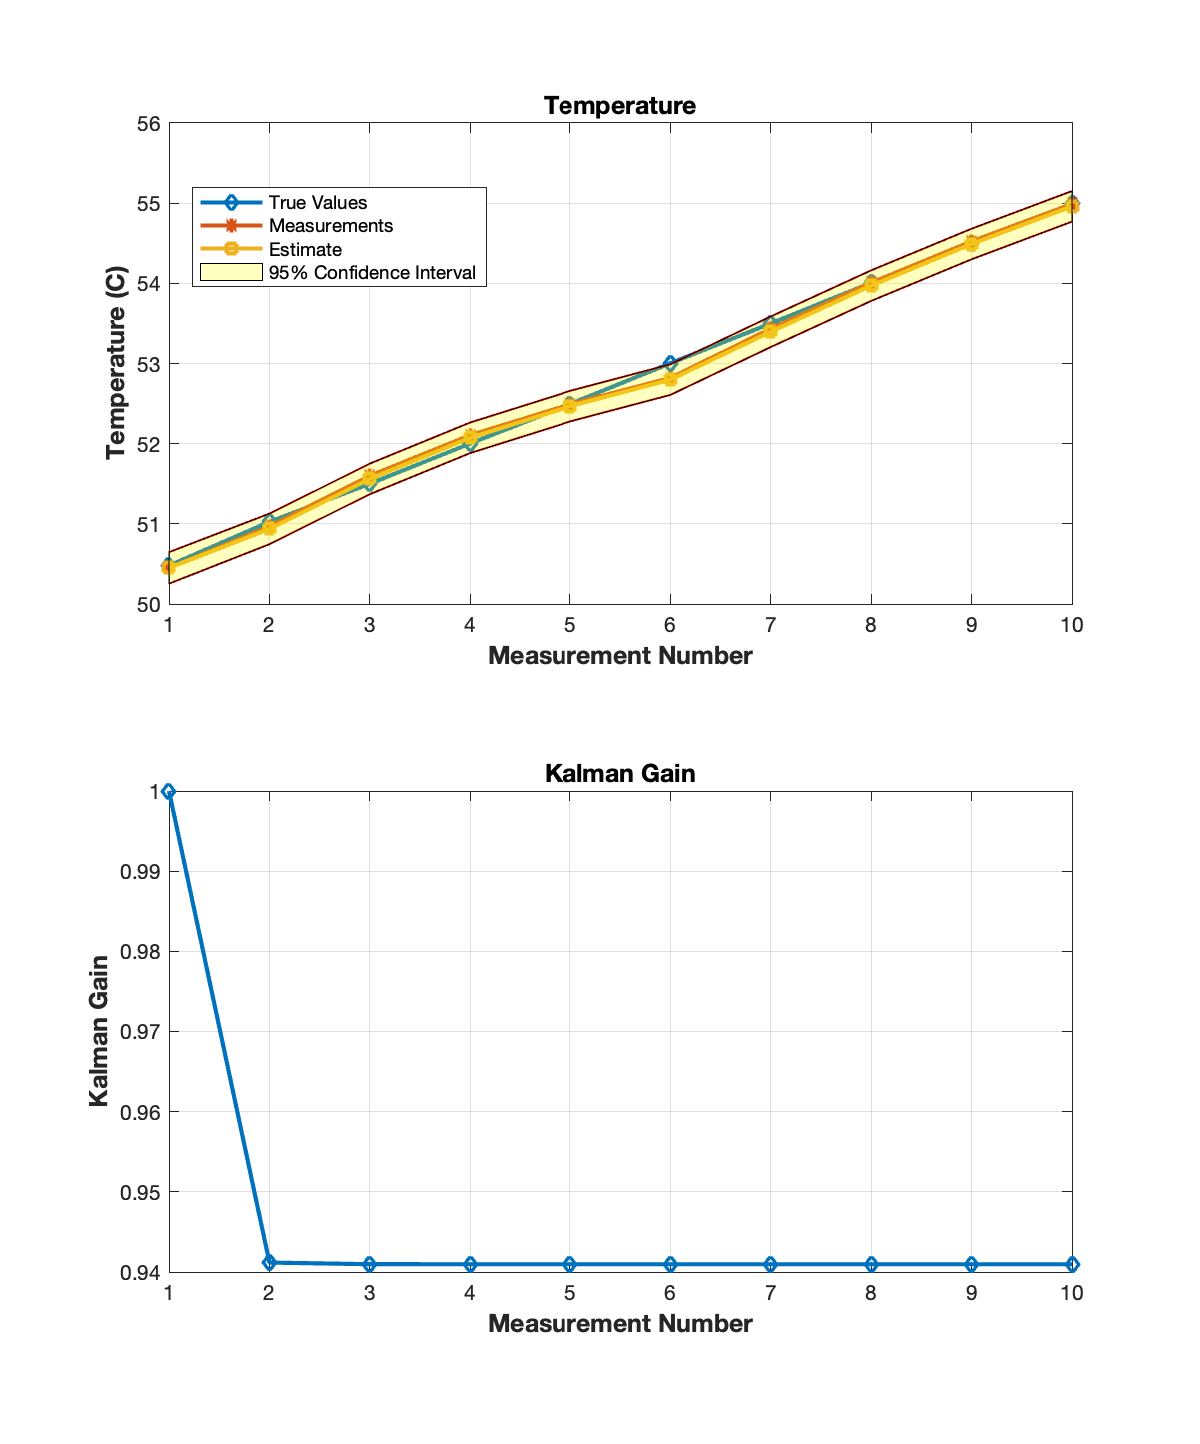
\includegraphics[width=1\textwidth]{Figures/Chapter1/ex8_KalmanFilter_ProcessNoise_II.eps}
    \label{fig:ex8_KalmanFilter_ProcessNoise_II}
    \vspace{-15pt}
    \end{figure}
        \texttt{\tiny [Code: 1D KF/Ex8\_KalmanFilter\_ProcessNoise\_II.m]}
\end{columns}
    
\end{frame}
